%%===========================================================%%
%%                                                           %%
%%       Data driven corrections to TPC/TOF efficienciy      %%
%%                                                           %%
%%===========================================================%%


\chapter{Corrections to efficiencies}\label{chap:tpcTofEffCorr}

\section{Data driven corrections to TOF efficiency}\label{sec:tofAbsEffCorr}

The efficiency of TOF hit reconstruction and matching with the TPC tracks that was used in our analyses was (at the very beginning) taken directly from the STAR simulation. This made the inaccuracies in the description of real detector geometry and its response propagating to physics results and introducing a bias. We decided to derive the correction to the TOF efficiency obtained from the STAR simulation by extracting it in the very same way from the data and embedded MC and comparing the results.% In this section we show the TOF efficiency analysis that led to derivation of the correction to the TOF efficiency and the systematic error of the latter.

% Unfortunately, in 2015 there were not enough data collected during low-luminosity runs (only production_pAl200_2015_lowlumi) that would imply lack of off-time pile-up tracks in TPC and thus would allow calculating the TOF efficiency in straightforward way, namely by dividing number of selected TPC tracks that were matched with TOF hits by number of all selected TPC tracks (matched or unmatched). Only y. 

For this purpose a variation of the ``tag and probe'' method was developed and used. This method utilizes some specific feature of the distribution of quantity describing two objects (whose trigger/reconstruction/identi- fication/etc. efficiency is studied) which allows to quantify amount of these objects with satisfied/unsatisfied efficiency condition. This could be e.g. $J/\psi$ peak in the invariant mass spectrum of the muon tracks, like in the study of muon identification efficiency in MTD~\cite{Huang:2016dbm}. %
%An example could be e.g. extraction of the muon identification efficiency in MTD. The quantity providing characteristic feature would be invariant mass of two opposite-sign tracks, which should contain a $J/\psi$ peak in the invariant mass spectrum for real muon tracks. One could tightly select one track likely being a muon (it would be a tag), and fill the histograms of $m(\mu^{+}\mu^{-})$ for all pairs tag+probe, where probes would be all tracks which 

%---------------------------
\begin{figure}[b!]%\vspace{-2pt}%
\centering%
\begin{minipage}{.4725\textwidth}%
  \centering%\vspace{11pt}
  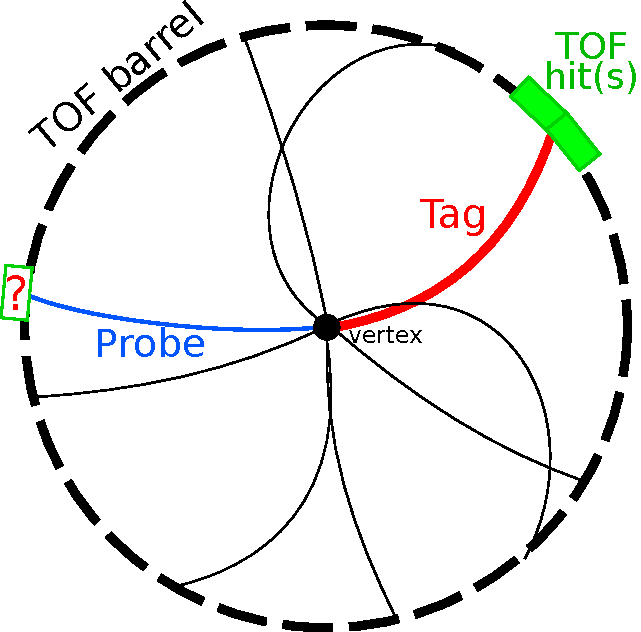
\includegraphics[width=0.98\linewidth]{graphics/correctionsToEff/TOF_tagAndProbe/sketch.pdf}%\vspace{-5pt}%
  \caption[Sketch of the tag\&probe method.]%
  {Sketch of the cross section of the central detector and CEP event with off-time pile-up tracks with drafted tag\&probe method used to determine the TOF hit reconstruction and matching efficiency. }\label{fig:tagAndProbeSketch}
\end{minipage}%
\quad\quad%
\begin{minipage}{.4725\textwidth}%
  \centering%
  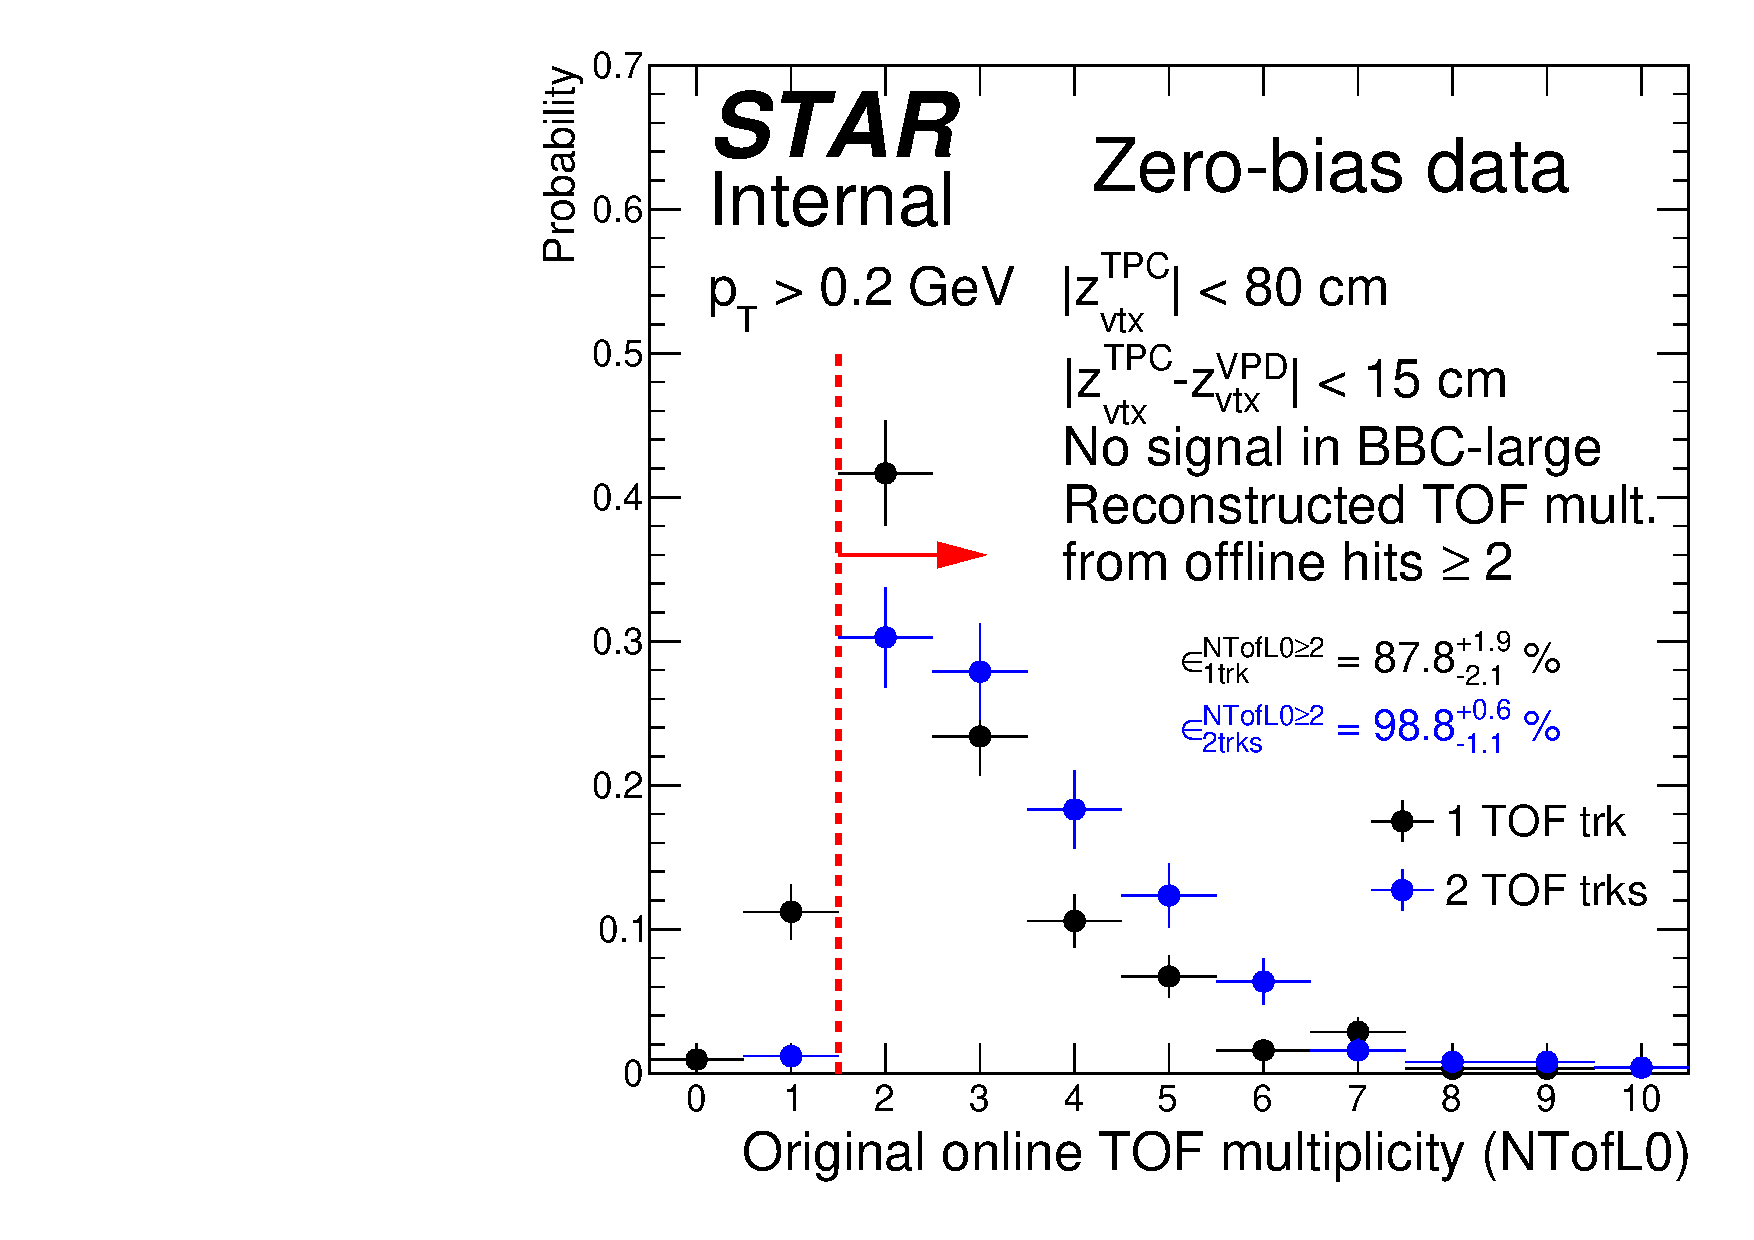
\includegraphics[width=\linewidth]{graphics/correctionsToEff/TOF_tagAndProbe/TofL0Eff_1TofVtx.pdf}%\vspace*{-5pt}
  \caption[TOF L0 multiplicity distribution for events with multiplicity reconstructed from offline hits $\geq 2$.]
   {TOF L0 multiplicity in events with exactly 1 (black) or exactly 2 (blue) primary TPC track matched with offline TOF hits under condition of online TOF mult. reconstructed from offline hits $\geq 2$.}%% Double-side VPD signal and veto in BBC-large required.
   \label{fig:tofTrigEffTagAndProbe}%\vspace*{-29pt}
\end{minipage}%
\end{figure}%
%--------------------------- 

In our varation of mentioned tag\&probe method the CEP of $\pi^{+}\pi^{-}$ events were used, with the missing transverse momentum $p_{T}^{\text{miss}}$ used to determine signal event yield ($p_{T}^{\text{miss}}=(\vec{p}_{W}+\vec{\pi}^{+}+\vec{\pi}^{-}+\vec{p}_{E})_{T}$). In short, events with forward proton track on each side of STAR and with a TOF-matched primary TPC track (tag) were selected. Among the remaining primary TPC tracks in the same vertex the opposite-sign TPC track (probe) was chosen as the one which provides the minimum total transverse momentum of all four tracks. The probe was checked whether it has been matched with the TOF hit or not. The ratio of the matched TPC tracks to all (matched or unmatched) TPC tracks defined the TOF efficiency, as given in Eq.~\eqref{eq:tagAndProbeEffDef}:%
\begin{equation}\label{eq:tagAndProbeEffDef}%
\varepsilon^{\text{TOF}}=\frac{N^{\text{probes}}_{\text{satisified}}}{N^{\text{probes}}_{\text{produced}}} = \frac{\textcolor{dgreen}{N^{\text{probes}}_{\text{satisified}}}}{\textcolor{dgreen}{N^{\text{probes}}_{\text{satisified}}}+\textcolor{red}{N^{\text{probes}}_{\text{failed}}}} = \frac{\textcolor{dgreen}{2 N^{\text{events}}_{TT}} + \textcolor{dgreen}{N^{\text{events}}_{TP_{s}}}}{\textcolor{dgreen}{2 N^{\text{events}}_{TT}} + \textcolor{dgreen}{N^{\text{events}}_{TP_{s}}} + \textcolor{red}{N^{\text{events}}_{TP_{f}}}}
\end{equation}%
Subscripts $TT$, $TP_{s}$ and $TP_{f}$ denote possible combinations of tags and probes:\\[-17pt]
\begin{itemize}%\scriptsize 
 \item $TT$ (both tracks satisfy tag criteria, and by definition the efficiency condition); such events provide two probes which satisfy efficiency condition which is the reason for the factor '2' in front of $N^{\text{events}}_{TT}$ in Eq.~\eqref{eq:tagAndProbeEffDef},\\[-17pt]
 \item $TP_{s}$ (one track is tag, the other is a probe and probe satisfies the efficiency condition),\\[-17pt]
 \item $TP_{f}$ (one track is tag, the other is a probe and probe fails to satisfy the eff. condition).%\\[-7pt]
\end{itemize}%
The method is illustrated in the sketch in Fig.~\ref{fig:tagAndProbeSketch}. The detailed description of the procedure of the TOF efficiency extraction is listed below:
%
%
%
%
%
%Since there is no simulation of the TOF trigger we assumed in MC analysis that any reconstructed offline TOF hit guarantees the L0 TOF multiplicity $\geq0$. In Fig.~\ref{fig:tofTrigEffTagAndProbe} we show that this assumption is safe. Appropriate correction is applied in the event weighting procedure, as explained later.
%
\begin{enumerate}
 \item Data from RP\_CPT2 trigger were used. This trigger required at least 2 level-0 TOF hits (trigger details can be found in Tab.~2.1 of Ref.~\cite{AnalysisNoteRafal}). Requirement of 2 TOF hits in the trigger (to ensure presence of 2 tracks in TPC) does not comply with the basics of the tag\&probe method, but as explained in \#4 and in the following page the tight selection of tags as tracks providing online multiplicity 2 and firing the TOF trigger allowed to use this method. GenEx $\pi^{+}\pi^{-}$ singnal MC (embedded into zero-bias data from runs corresponding to RP\_CPT2 triggers), as well as Pythia CD for non-exclusive background, were subjected to the same trigger conditions, except online TOF multiplicity condition to avoid trigger bias. Trigger bias present in the data was removed by applying correction obtained from Fig.~\ref{fig:tofTrigEffTagAndProbe} and described in text.\\[-20pt]% in the text.
 %
%  Tu trzeba opisać, że wprawdzie wymóg  dwóch hitów w TOF na poziomie trygera łamie podstawy metody tag&probe to jednak selekcja tagów które z wysokim prawdopodobieństwem  zapewniają samodzielnie wyzwolenie trygera umożliwia stosowanie tej metody.
 \item Events were selected with the cuts from nominal CEP analysis (Ref.~\cite{AnalysisNoteRafal}), except cuts \textbf{C3} and \textbf{C7-C9} which were removed or modified as given below. This provided significant reduction of background events.\\[-20pt]%
 %
 \item For each event passing above selection primary TOF-matched TPC tracks of good quality (cuts~\ref{sec:TpcQualityCuts},\ref{sec:TpcDcaCuts}), contained within kinematic region of our measurement (cuts~\ref{sec:TpcKinematicCuts} with $p_{T}$ threshold lowered to 0.18~GeV to also calculate efficiency in a point where it rapidly changes hence allow more precise fit to efficiency $p_{T}$-dependece) and compatible with pion hypothesis based on $dE/dx$ ($|n^{\sigma}_{\text{pion}}|<3$) were selected. If any TOF-matched track incompatible with pion hypothesis was found, event was dropped from analysis. Also, event was not analyzed if more than 2 TOF-matched tracks were reconstructed (not two-prong CEP event).\\[-20pt]%
 %
 \item Primary TOF-matched TPC tracks preselected in \#3 were set as tag candidates. In the data they were additionaly required to be matched with the TOF hit belonging to a TOF cluster that is expected to provide multiplicity 2 at the level 0 (to reduce trigger bias). In case only one track was found to be a tag candidate, steps \#5-\#6 were executed only with this single track being a tag. Otherwise steps \#5-\#6 were repeated for each of two tracks set as a tag.\\[-20pt]%
 %
 \item From the remaining TPC tracks in the same vertex (preselected in \#3) of the sign opposite to tag and of good quality (cuts~\ref{sec:TpcQualityCuts},\ref{sec:TpcDcaCuts}), the one which provided the best transverse momentum balance together with 2 protons and a tag was selected as a probe (signature of exclusive $\pi^{+}\pi^{-}$ is  $p_{T}^{\text{miss}}\sim0$). If no primary TPC tracks passing this selection were found, an event was dropped.\\[-20pt]%
 %
 \item 2-dimensional histograms of quantities of interest $q$ (probe $\eta$, probe $p_{T}$, $z_{\text{vtx}}$) vs. $p_{T}^{\text{miss}}$ were filled, separately for all probes and only for probes matched with TOF. Each probe (each entry to the histogram) was associated with the weight $w$ taking into account the trigger efficiency and vertexing efficiency, as given in Eq.~\eqref{eq:tagAndProbeWeight} and explained later in the text.\\[-20pt]%
 %
 \item In each bin of quantity of interest $q$ (as a function of which the efficiency was to be determined) the distribution of $p_{T}^{\text{miss}}$ was fitted in the signal-free region with the function describing background shape. The background function was extrapolated to $p_{T}^{\text{miss}}=0$. The signal yield in given bin of $q$ was calculated as the integral of the histogram with subtracted integral of the background function, both in the range $p_{T}^{\text{miss}}<75$~MeV. The final efficiency in given bin of $q$ was calculated according to Eq.~\eqref{eq:tagAndProbeEffDef2}:%\vspace{-4pt}
 \begin{equation}\label{eq:tagAndProbeEffDef2}
  \varepsilon^{\text{TOF}}(q) = \frac{N_\text{weighted}^{\text{matched},~p_{T}^{\text{miss}}<75~\text{MeV}} - N_\text{bkgd,weighted}^{\text{matched},~p_{T}^{\text{miss}}<75~\text{MeV}} }{ N_\text{weighted}^{\text{all},~p_{T}^{\text{miss}}<75~\text{MeV}} - N_\text{bkgd,weighted}^{\text{all},~p_{T}^{\text{miss}}<75~\text{MeV}} }\vspace*{-25pt}
 \end{equation}
\end{enumerate}
%
%  
%
%
%
%
%
%---------------------------
\begin{figure}[h]\vspace*{5pt}
\centering
\parbox{0.4725\textwidth}{
  \centering
  \begin{subfigure}[b]{\linewidth}{
                \subcaptionbox{\label{fig:sampleMissingPtTagAndProbe_DATA}}{\includegraphics[width=\linewidth,page=8]{graphics/correctionsToEff/TOF_tagAndProbe/Fitting_effVsPt_data.CPT2.pdf}\vspace{-15pt}}}
  \end{subfigure}
}
\quad
\parbox{0.4725\textwidth}{
  \centering
    \begin{subfigure}[b]{\linewidth}{
                \subcaptionbox{\label{fig:sampleMissingPtTagAndProbe_MC}}{\includegraphics[width=\linewidth,page=8]{graphics/correctionsToEff/TOF_tagAndProbe/Fitting_effVsPt_mc.CPT2.pdf}\vspace{-15pt}}}
  \end{subfigure}
}\vspace{-5pt}%
\caption[Sample distributions of $p_{T}^{\text{miss}}$ of the $p$+Tag+Probe+$p$ system in the data and embedded MC.]%
    {Sample distributions of total transverse momentum $p_{T}^{\text{miss}}$ of the $p$+Tag+Probe+$p$ system in the data (\ref{fig:sampleMissingPtTagAndProbe_DATA}) and signal+background embedded MC (\ref{fig:sampleMissingPtTagAndProbe_MC}). TOF-matched and all (matched or unmatched) probes are represented by histograms in green and black color, respectively. The red dashed line shows the exclusivity cut value ($75~\text{MeV}/c$). Signal yield is determined via the integral of the histogram with subtracted integral of the solid line representing non-exclusive background in the $p_{T}^{\text{miss}}$ range to the left from the vertical line. Background (solid line) is fitted with 2$^{\text{nd}}$ order polynomial in the signal-free region (the details can be found in Ref.~\cite{AnalysisNoteRafal} in Sec.~5.2). Full sets of histograms in different ranges of probe $p_{T}$ and $\eta$ are included in Appendix~\ref{appendix:tagAndProbeTofEff}.}\label{fig:sampleMissingPtTagAndProbe}%
\end{figure}
%---------------------------
\newpage%
%
As described in the algorithm of the tag\&probe method, the RP\_CPT2 triggers were used in our study. The logic of that trigger required at least 2 TOF hits online. Since the system whose efficiency was studied has also been a part of the trigger, the tag should be, in principle, chosen as the track that is linked with 2 online TOF hits - to be sure that the tag satisfies the trigger condition and thus the probe is not biased by the trigger (in other words, the probe does not bias the resultant efficiency). Unfortunately, the TOF system works independently for the trigger and for the offline data stream (the readout electronics are independent), therefore there is no information about the connection between the TOF hits at L0 and offline.
 
Fortunately, a solution to the above limitation has been found. We made use of the TOF cluster\footnote{Group of offline TOF hits adjacent/close to each other in space (and time)} concept introduced in Ref.~\cite{AnalysisNoteRafal},~Sec.XX, as well as of reconstruction/emulation of the online TOF multiplicity from the offline hits according to description of the TOF trigger system in Ref.~\cite{tofL0MultExplanation}. With these tools we chose tags as the tracks that are matched with TOF hit associated with a TOF cluster that provides reconstructed online multiplicity $\geq 2$. We verified with zero-bias data that by requiring the reconstructed online multiplicity to be $\geq 2$ we can efficiently select events in which the true online (L0) TOF multiplicity was also $\geq 2$. For this purpose we selected events with only one(two) TOF-matched TPC track(s), in addition forming a primary vertex. We also required no signal in large BBC tiles, the same as in physics analysis of CEP. To make sure that the single TOF-matched track is from beam-beam interaction that TOF electronics is adjusted to trigger on, we required the signal in VPD detectors on both sides of the IP. The $z$-positions of the primary vertex reconstructed in TPC and reconstructed from the time difference in west and east VPDs was required to be not larger than 15~cm. In Fig.~\ref{fig:tofTrigEffTagAndProbe} we show distribution of the TOF L0 multiplicity for such selected events. One can find in this figure that the probability of TOF L0 multiplicity $\geq 2$ for a single TOF-matched track, $\epsilon^{\text{NTofL0}\geq2}_{1\text{trk}}$, is high and equals 87.8\%. For events with 2 reconstructed TOF-matched tracks the probability of TOF L0 multiplicity $\geq 2$, $\epsilon^{\text{NTofL0}\geq2}_{2\text{trks}}$, equals 98.8\%. These efficiency factors were accounted in the event weighting, as shown in Eq.~\eqref{eq:tagAndProbeWeight}.
 
The vertexing efficiency was an additional efficiency factor which had to be taken into account in described analysis\footnote{This analysis could be performed using solely global TPC tracks without requiring reconstructed primary vertex. Such solution was not chosen due to limitation of the picoDST data accessible for analysis (not all global tracks stored).}. This efficiency for a single track depends on matching with TOF due to 'useBTOFmatchOnly' option used in reconstruction. %
%
%---------------------------
\begin{figure}[b!]
\centering
\parbox{0.4725\textwidth}{
  \centering
  \begin{subfigure}[b]{\linewidth}
                \subcaptionbox{\label{fig:vertexingEffVsD0}}{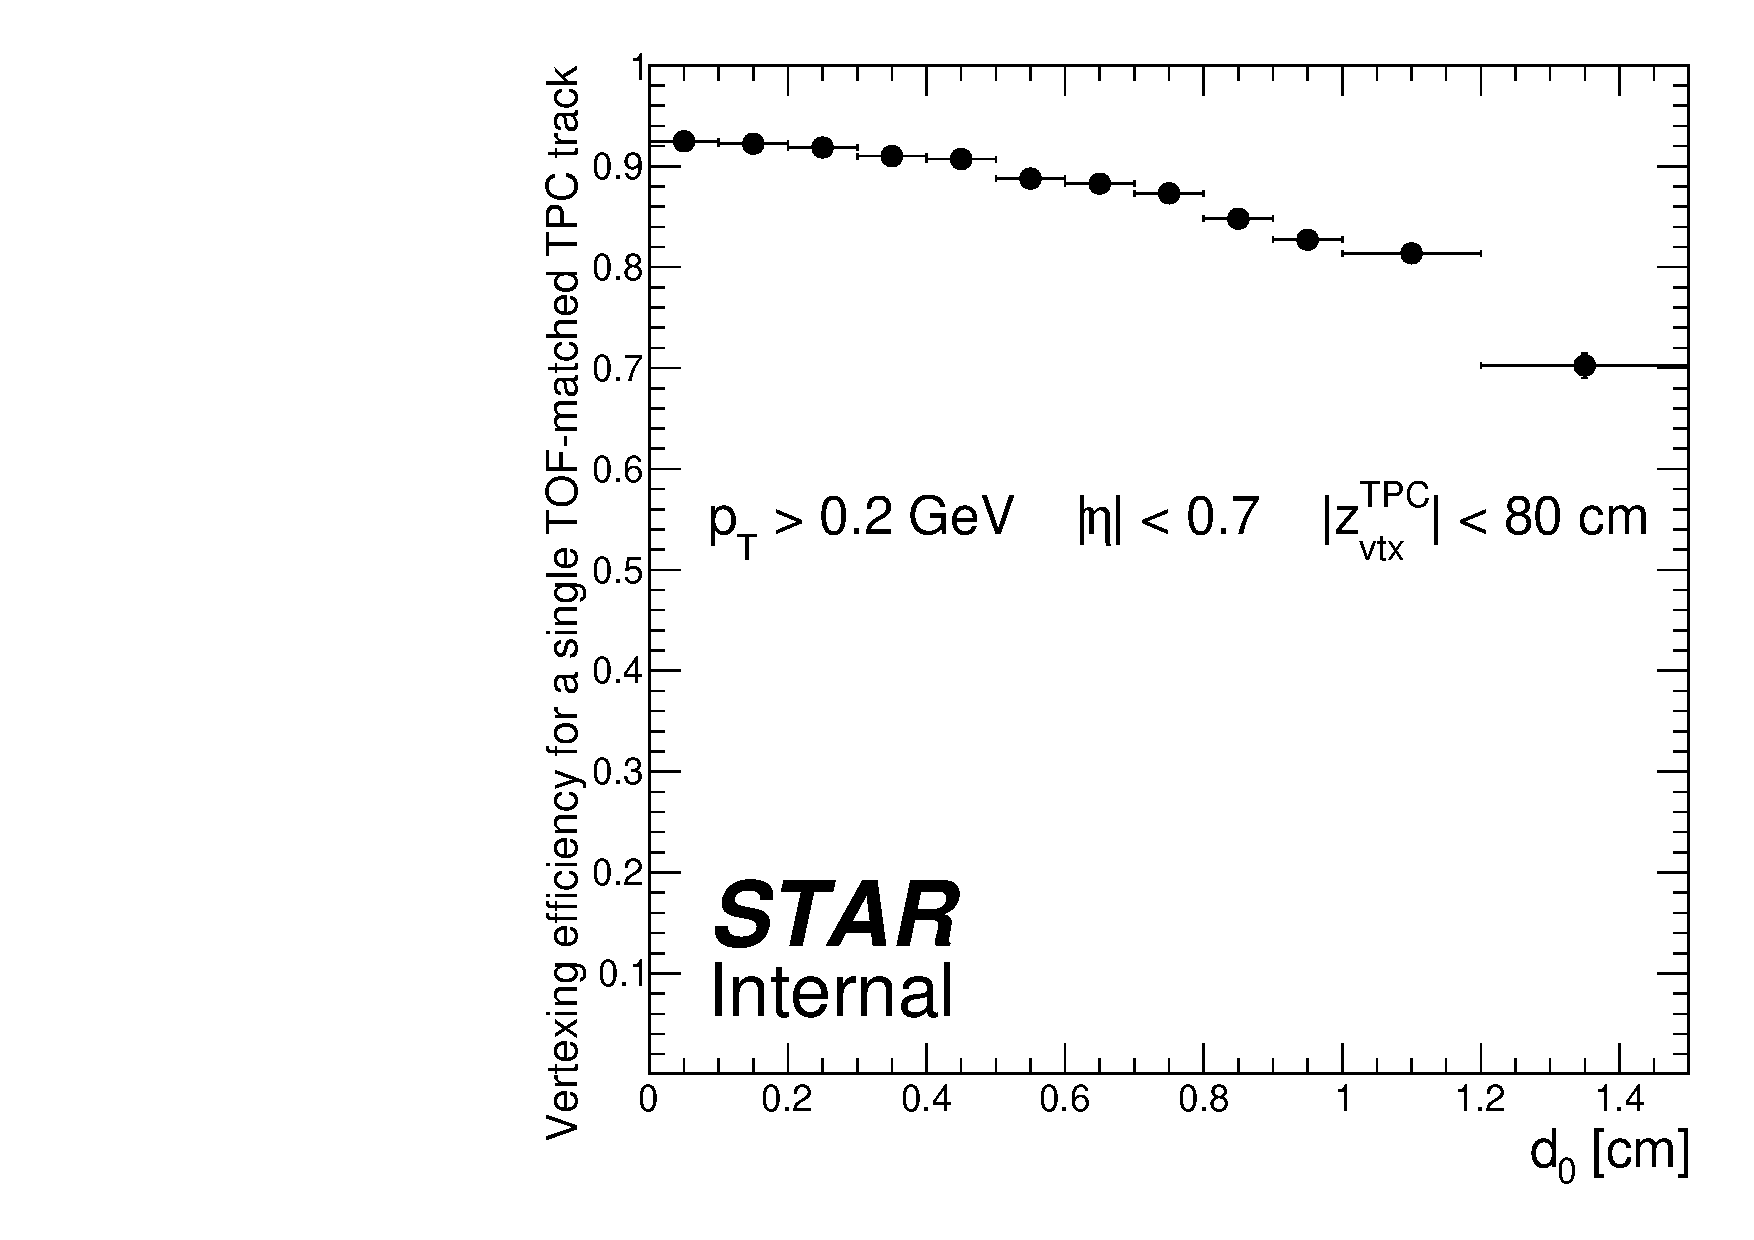
\includegraphics[width=\linewidth]{graphics/correctionsToEff/TOF_tagAndProbe/VertexingEffVsD0.pdf}\vspace{-8pt}}\vspace{-5pt}
  \end{subfigure}
}%
\quad\quad%
\parbox{0.4725\textwidth}{
  \centering
  \begin{subfigure}[b]{\linewidth}
                \subcaptionbox{\label{fig:vertexingEff2D}}{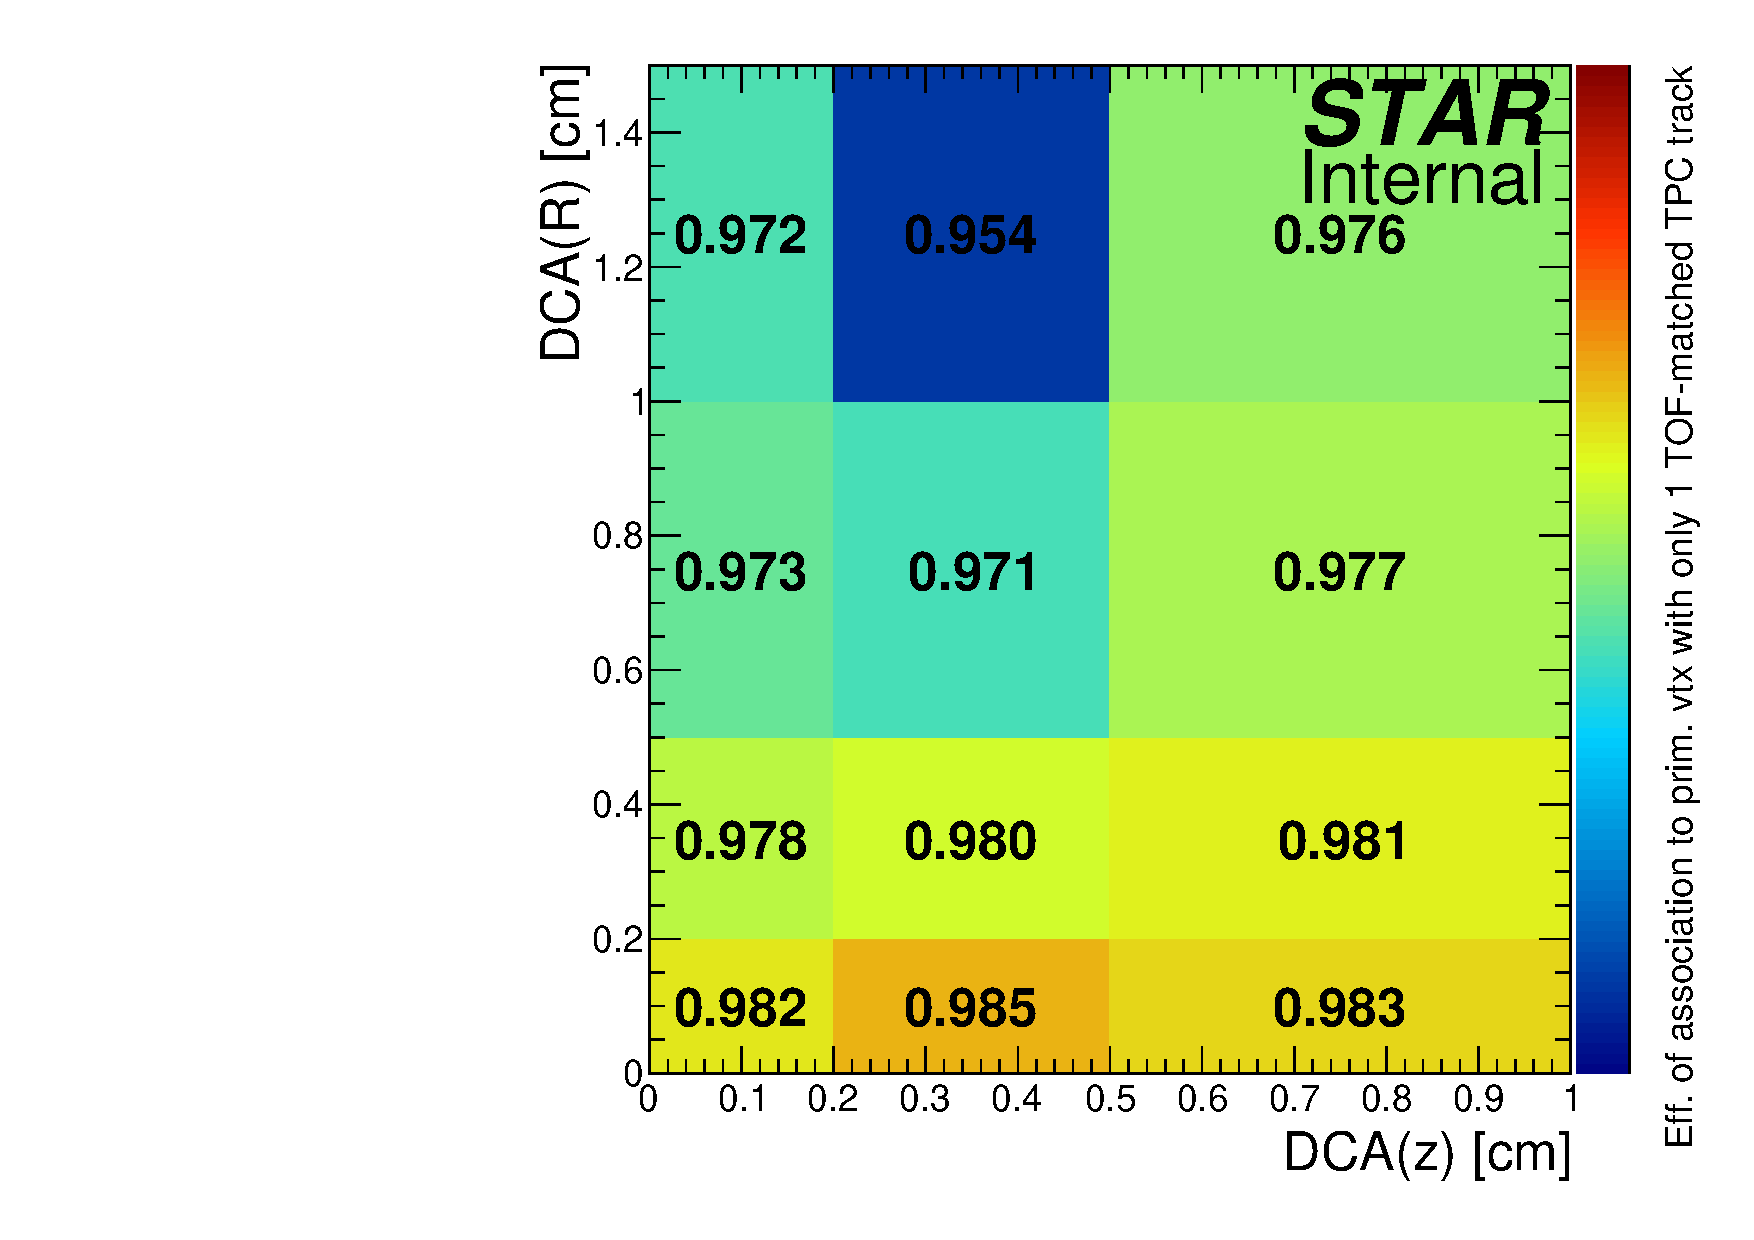
\includegraphics[width=\linewidth]{graphics/correctionsToEff/TOF_tagAndProbe/VertexingEffVsDCA_2D.pdf}\vspace{-8pt}}\vspace{-5pt}
  \end{subfigure}
}%
\caption[Efficiencies for reconstruction of the vertex with single TOF-matched TPC track and association with this vertex of TOF-unmatched track.]%
    {Efficiency $\varepsilon_{vtx}^{\text{nTOF=1}}$ of reconstruction of the primary vertex from a single TOF-matched TPC track as a function of the absolute value of the transverse impact parameter $d_{0}$ (\ref{fig:vertexingEffVsD0}) and efficiency $\varepsilon_{vtx}^{\text{no-TOF}}$ of association with the vertex formed from single TOF-matched track of a TPC track not matched with TOF, as a function of radial and longitudinal DCA to the vertex (\ref{fig:vertexingEff2D}). The tracks were required to be matched with true-level primary particles (pions) as well as the quality and kinematic cuts were implied (\ref{sec:TpcQualityCuts}, \ref{sec:TpcDcaCuts}, \ref{sec:TpcKinematicCuts}).}\label{fig:vertexingEffTagAndProbe}%
\end{figure}
%---------------------------
%
%
It is different when both exclusive pion tracks are matched with TOF, comparing with the case when only one track is matched with TOF and the other is not. The vertexing efficiency defined as the probability that two global TPC tracks of true-level primary particles, matched with TOF and satisfying criteria \ref{sec:TpcQualityCuts}, form the common primary vertex is presented in Ref.~\cite{AnalysisNoteRafal} in Fig.XXX as a function of the distance in $z$ of the DCA points on the beamline, $|\Delta z_{0}|$. This efficiency extracted from embedded MC was used in this analysis in case when both tag and probe were matched with TOF. As shown in dedicated study presented in Ref~\cite{AnalysisNoteRafal} in Sec.XXX, the MC reproduces very well the vertexing efficiency obtained from the data.

For events with only one of exlusively produced pions being matched with TOF a different efficiency had to be used. In this case only the TOF-matched track participated in the vertexing, while the other was added to the primary vertex if it satisfied certain criteria. We therefore calculated the vertexing efficiency for the single TOF-matched track as a function of the transverse distance to the beamline $|d_{0}|$ (Fig.~\ref{fig:vertexingEffVsD0}) and the efficiency of association of the TPC track not matched with TOF with the primary vertex made of single TOF-matched track (Fig.~\ref{fig:vertexingEff2D}). The final correction factor for a probe represented by the weight of an entry to $q$~vs.~$p_{T}^{\text{miss}}$ histograms has the following form:

\begin{equation}\label{eq:tagAndProbeWeight}%
w=\left\{
\begin{array}{ll}
\Big[\epsilon^{\text{NTofL0}\geq2}_{1\text{trk}}~\times~\varepsilon_{vtx}^{\text{nTOF=2}}(|\Delta z_{0}|)\Big]^{-1} & \textrm{for~}TT,~TP_{s}\\[3pt]
\Big[\epsilon^{\text{NTofL0}\geq2}_{2\text{trks}}~\times~\varepsilon_{vtx}^{\text{nTOF=1}}(|d_{0}|)\times \varepsilon_{vtx}^{\text{no-TOF}}(\text{DCA}_{z},\text{DCA}_{R})\Big]^{-1} & \textrm{for~}TP_{f}
\end{array}
\right.,
\end{equation}
where factors related to trigger efficiency are accounted only in the data analysis. A sample histograms of the $p_{T}^{\text{miss}}$ distribution in the data and embedded MC filled with entries of weight $w$ are shown in Fig.~\ref{fig:sampleMissingPtTagAndProbe}.

The dependence of the TOF efficiency on the track $p_{T}$ was assumed to have the error function (erf) form:
\begin{equation}\label{eq:tofEffFunc}
 \varepsilon^{\text{TOF}}(p_{T}) = \frac{1}{2} \cdot P_{1}\cdot  \Big(\text{erf}\Big(\frac{p_{T}-P_{2}}{P_{3}}\Big) + 1\Big)
\end{equation}

In Fig.~\ref{fig:tofEffSyst} we show the resultant TOF efficiency obtained with the Tag\&Probe method.

%---------------------------
\begin{figure}[h!]
\centering
\parbox{0.4725\textwidth}{
  \centering
  \begin{subfigure}[b]{\linewidth}{
                \subcaptionbox{\label{fig:tofEffSystVsPt_CPT}}{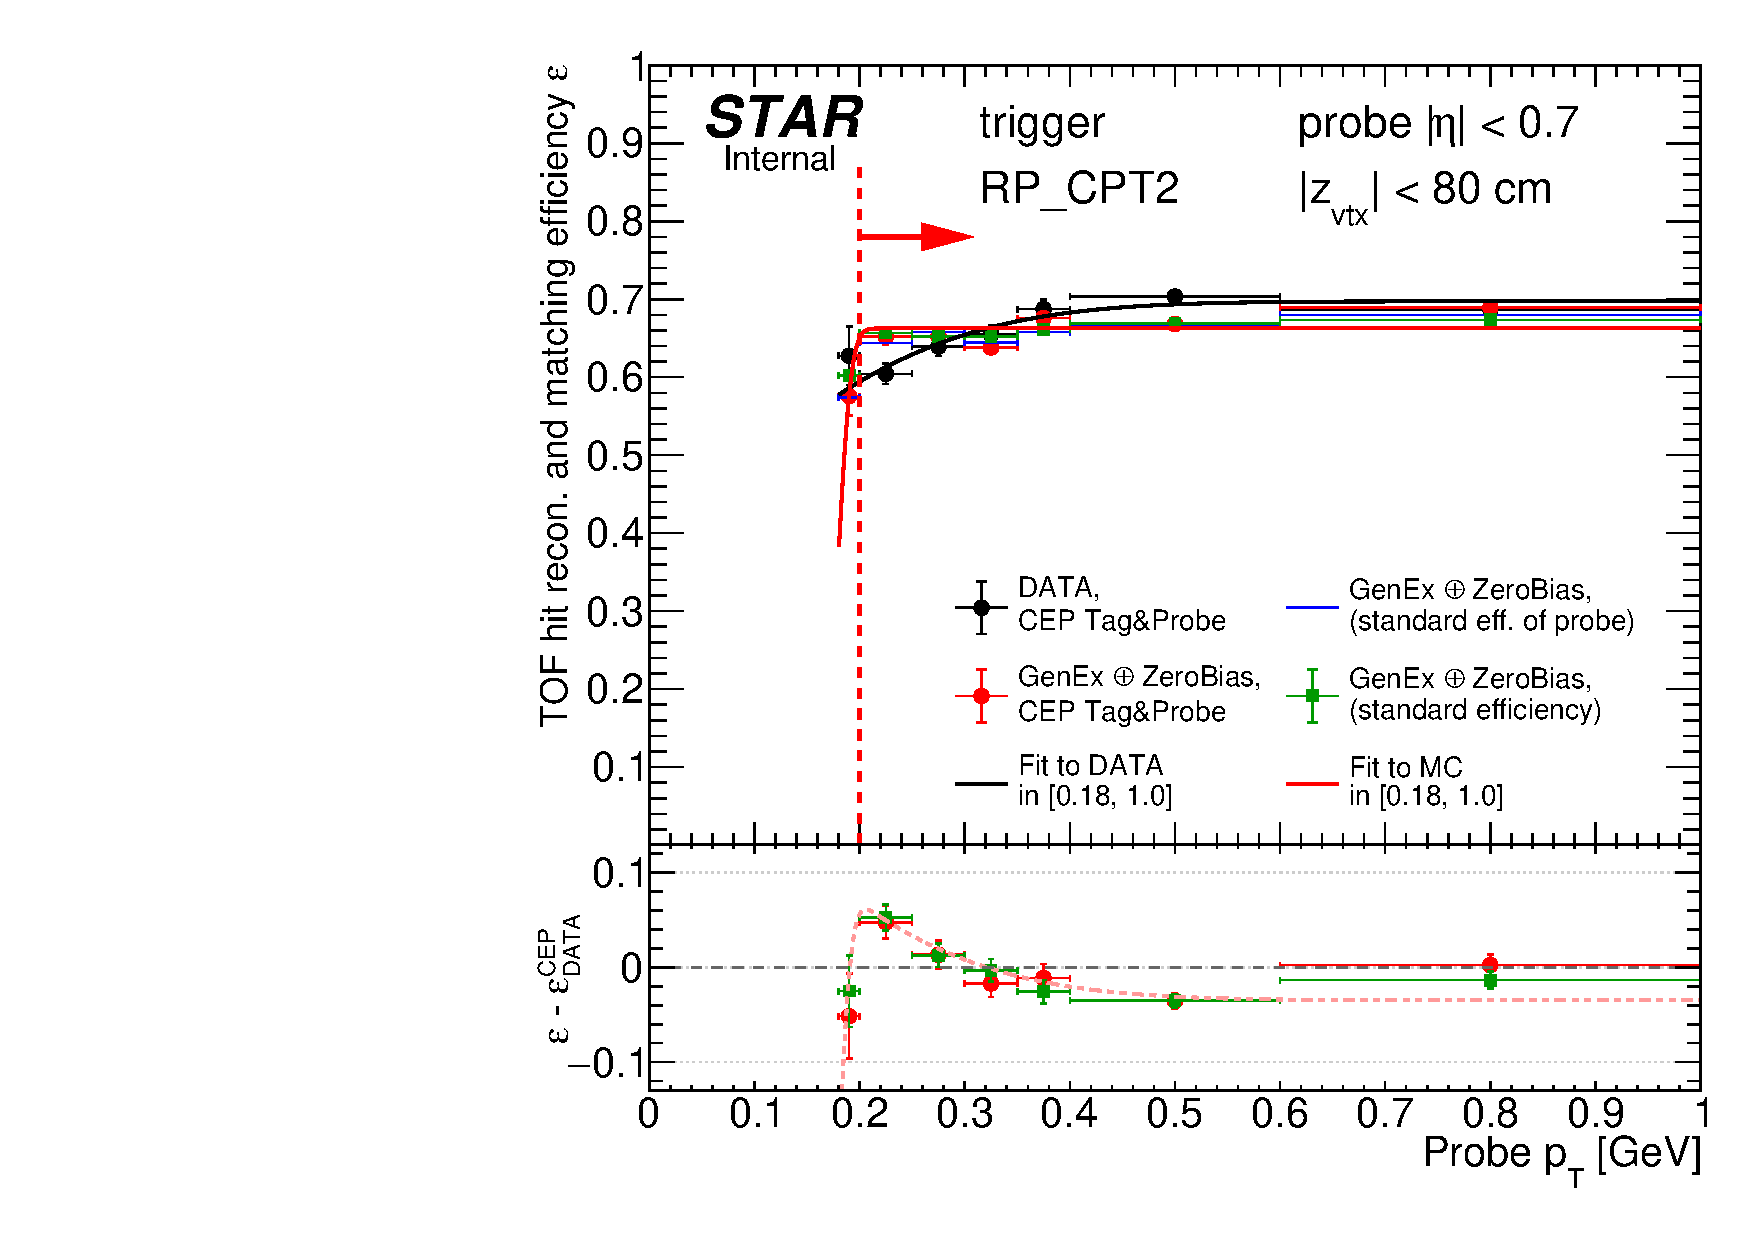
\includegraphics[width=\linewidth]{graphics/correctionsToEff/TOF_tagAndProbe/TofEffVsPt.CPT2.pdf}\vspace{-5pt}}}
  \end{subfigure}\\[5pt]
  \begin{subfigure}[b]{\linewidth}\addtocounter{subfigure}{1}{
                \subcaptionbox{\label{fig:tofEffSystVsZVtx_CPT}}{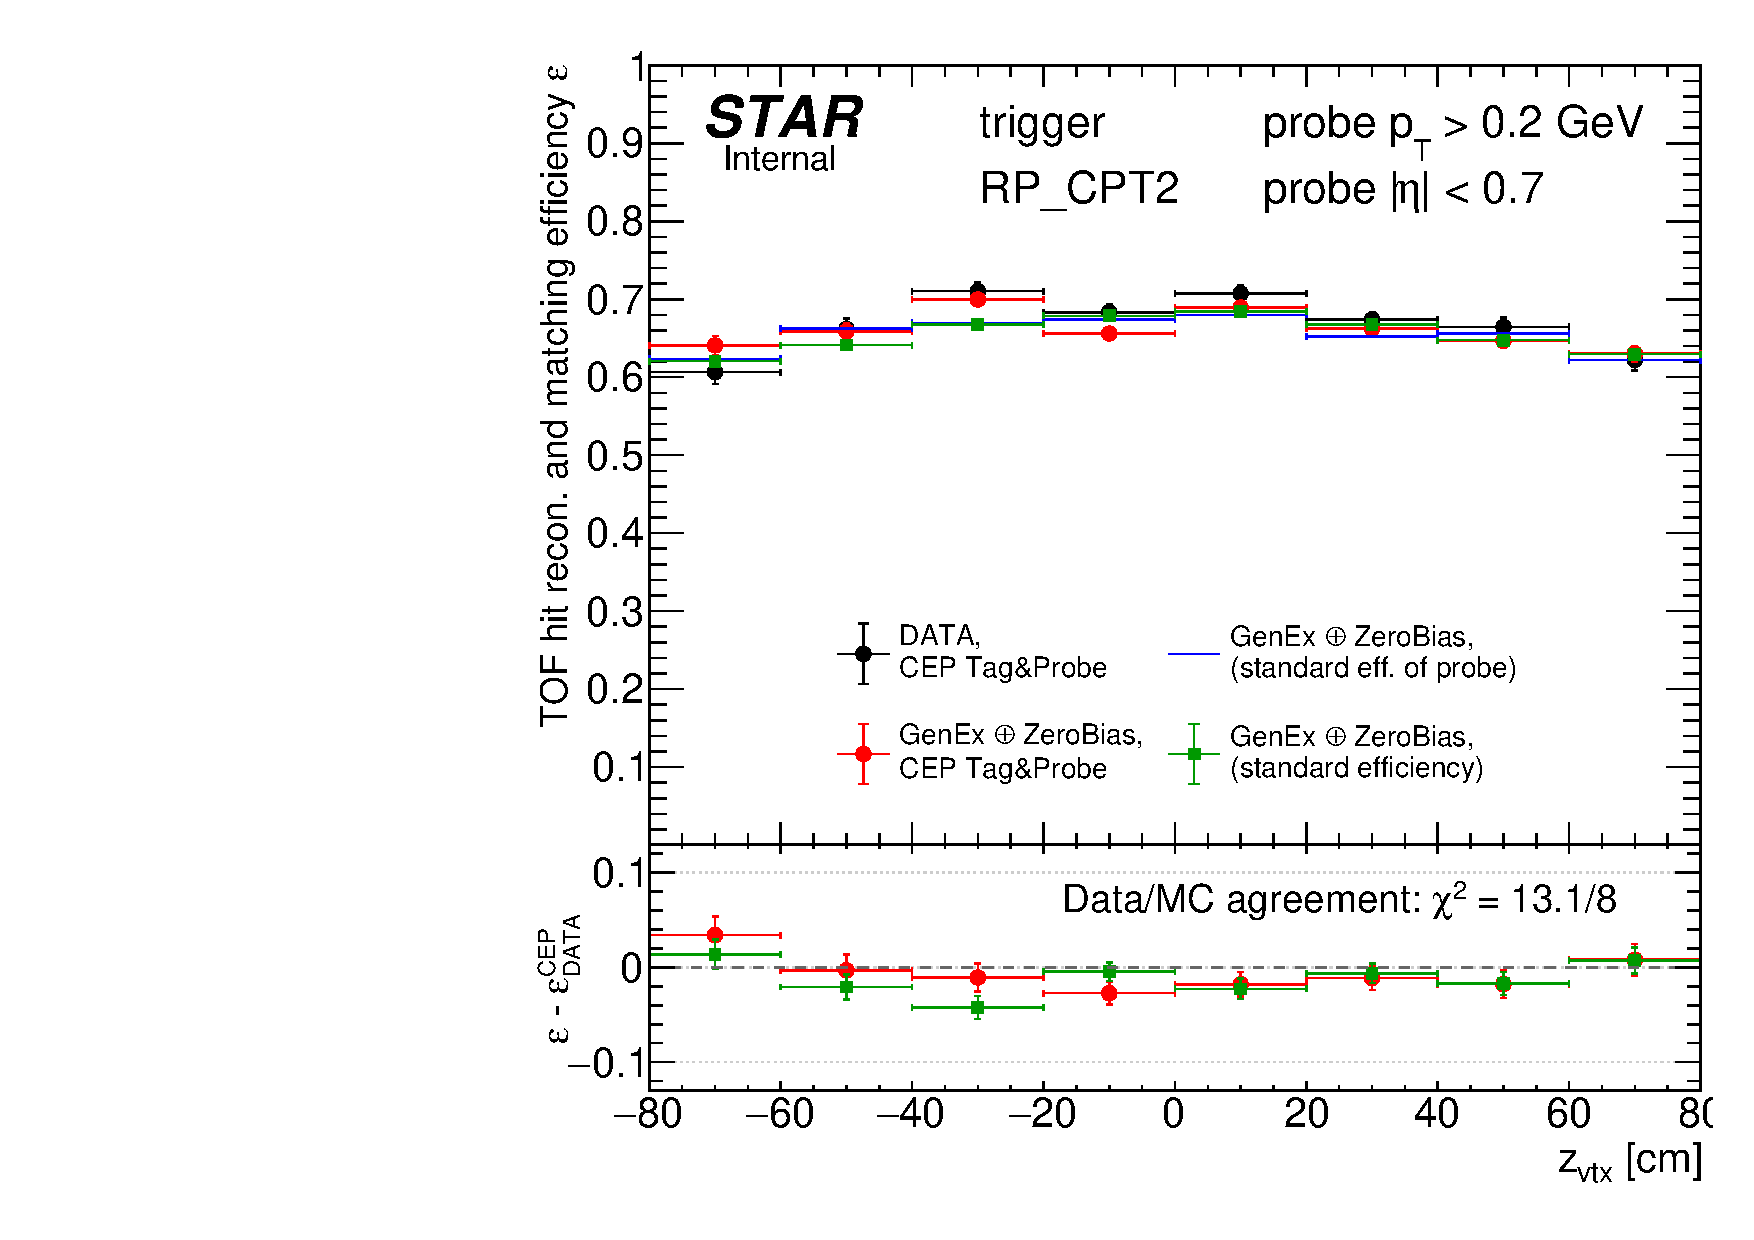
\includegraphics[width=\linewidth]{graphics/correctionsToEff/TOF_tagAndProbe/TofEffVsZVtx.CPT2.pdf}\vspace{-5pt}}}
  \end{subfigure}  
}
\quad
\parbox{0.4725\textwidth}{
  \centering\vspace*{-55pt}
    \begin{subfigure}[b]{\linewidth}\addtocounter{subfigure}{-2}{
                \subcaptionbox{\label{fig:tofEffSystVsEta_CPT}}{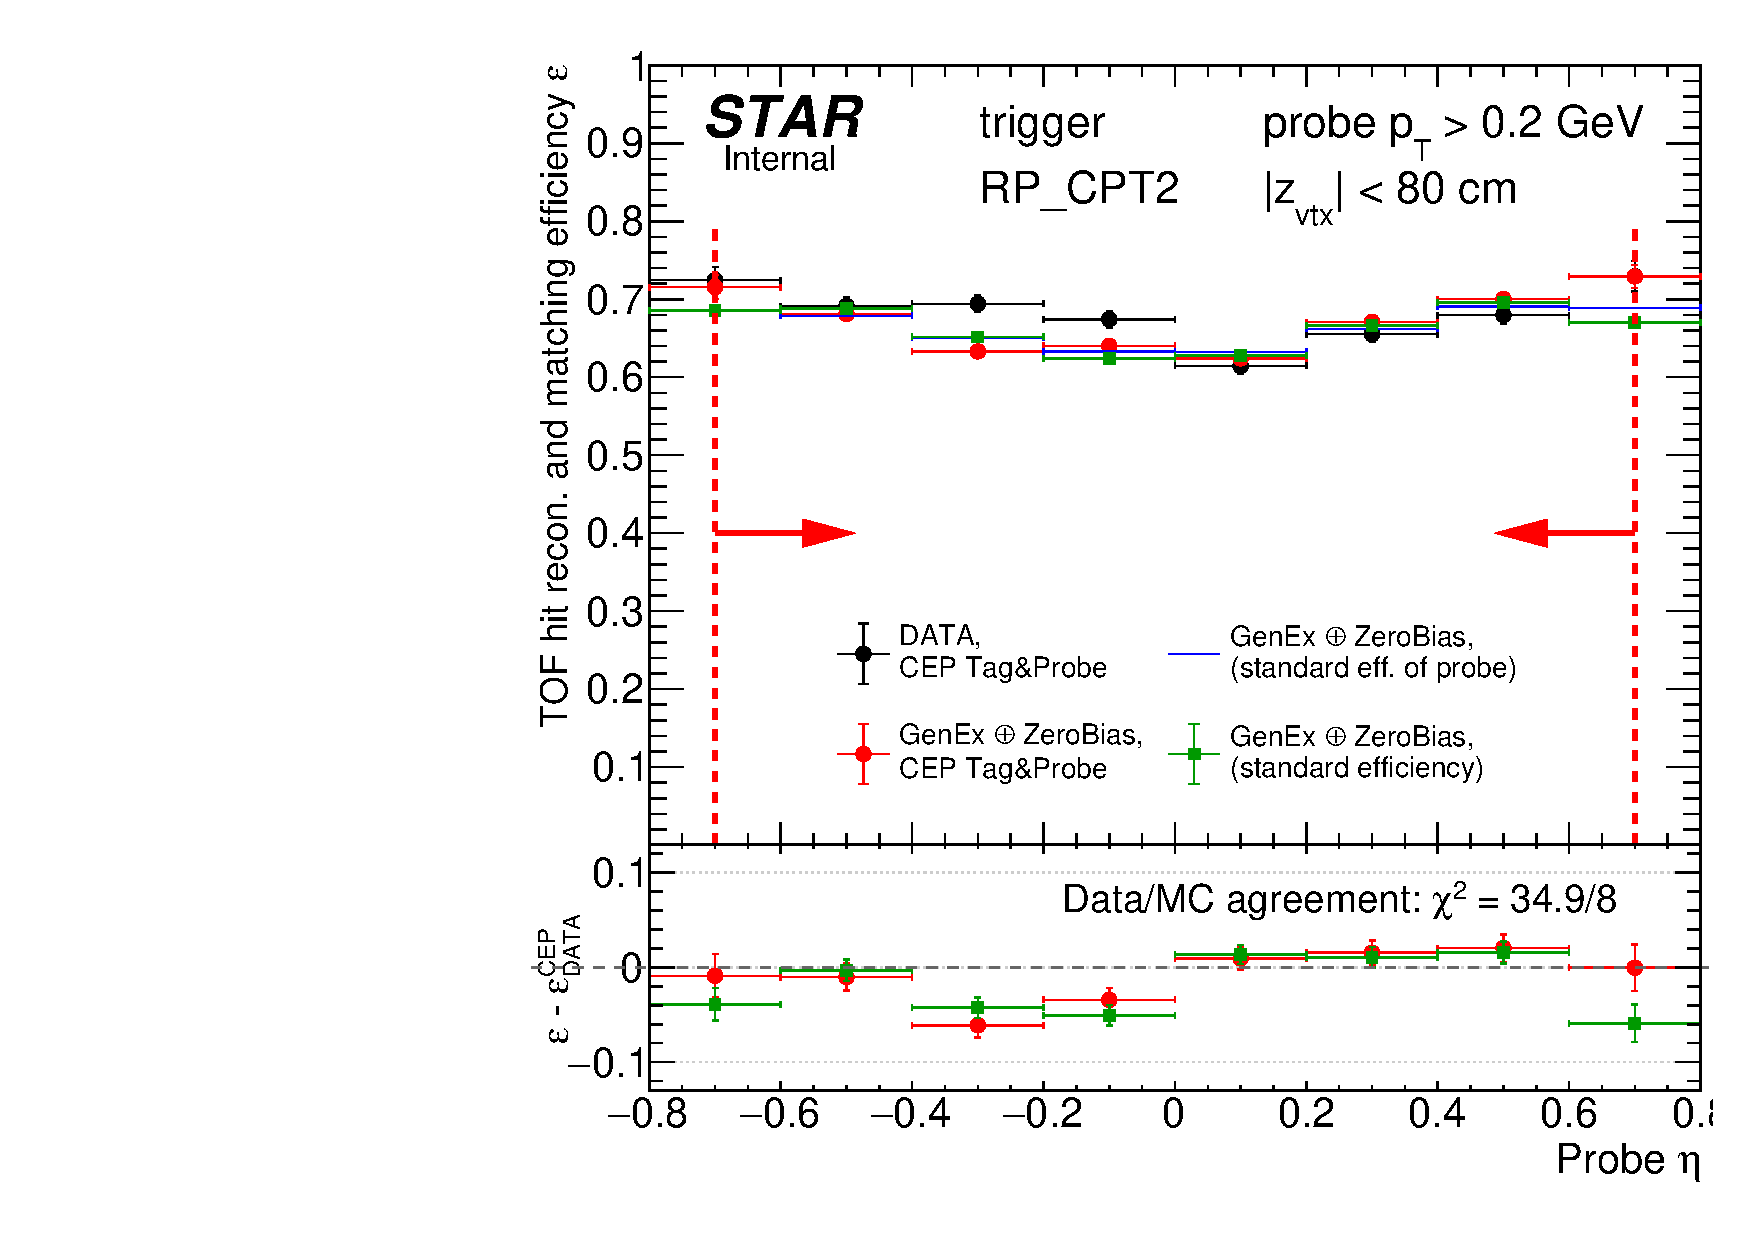
\includegraphics[width=\linewidth]{graphics/correctionsToEff/TOF_tagAndProbe/TofEffVsEta.CPT2.pdf}\vspace{-5pt}}}
  \end{subfigure}\\[5pt]
		\begin{minipage}[t][0.78\linewidth][t]{\linewidth}\vspace{10pt}
			\caption[Tag\&Probe TOF efficiency from CEP data compared with the result from embedded CEP MC.]%
    {Tag\&Probe TOF efficiency from CEP data (black points) compared with the result from embedded CEP MC (red points) as a function of TPC track $p_{T}$ (\ref{fig:tofEffSystVsPt_CPT}), $\eta$ (\ref{fig:tofEffSystVsEta_CPT}) and $z_{\text{vtx}}$ (\ref{fig:tofEffSystVsZVtx_CPT}). Green points represent the TOF efficiency calculated in the standard way from embedded CEP MC sample. Blue lines denote the TOF efficiency calculated in the standard way solely from the selected probe tracks that were matched to primary pions at the true level. Difference between red points and blue lines show the potential bias of tag and probe method. Solid lines are fits of function given by Eq.~\eqref{eq:tofEffFunc} to points of corresponding color. Dashed vertical lines with arrows indicate region of $p_{T}$ and $\eta$ accepted in analyses.}\label{fig:tofEffSyst}%
		\end{minipage}
} \vspace{-5pt}%
\end{figure}
%---------------------------



From Fig.~\ref{fig:tofEffSyst} one can find that the efficiency in the data and MC differ substantially. The comparison of the $p_{T}$-dependence of TOF efficiency in Fig.~\ref{fig:tofEffSystVsPt_CPT} suggests that saturation of the TOF efficiency with growing track $p_{T}$ is slower than MC predicts, and that maximum (high-$p_{T}$) efficiency is generally higher by 3-4 percentage points in the data compared to MC. In the $\eta$-dependence we can see that there are some bins of $\eta$ in which the agreement between MC and data is satisfactory, while in others the difference is large. The $z_{\text{vtx}}$-dependence (Fig.~\ref{fig:tofEffSystVsZVtx_CPT}) is in acceptable agreement between the data and MC.

The above observations led to perform the analysis of $p_{T}$-dependece of TOF efficiency in 4 bins of track pseudorapidity. The result is presented in Fig.~\ref{fig:tofEffSyst_etaBins}. Parameters of functions fitted to data anc MC points are contained in Tab.~\ref{tab:tofEffCorrParams}. The additive correction to the TOF efficiency presented in Sec.~\ref{sec:tofMatchEff} has the form
\begin{equation}\label{eq:tofEffCorr}
 \delta\varepsilon^{\text{TOF}}(p_{T}) = \varepsilon^{\text{TOF}}_{\text{DATA}}(p_{T}) - \varepsilon^{\text{TOF}}_{\text{MC}}(p_{T}),
\end{equation}%
%
%
%---------------------------
\begin{figure}[H]
\centering
\parbox{0.4725\textwidth}{
  \centering
  \begin{subfigure}[b]{\linewidth}{
                \subcaptionbox{\label{fig:TofEffVsPt_eta_minus07_to_minus03}}{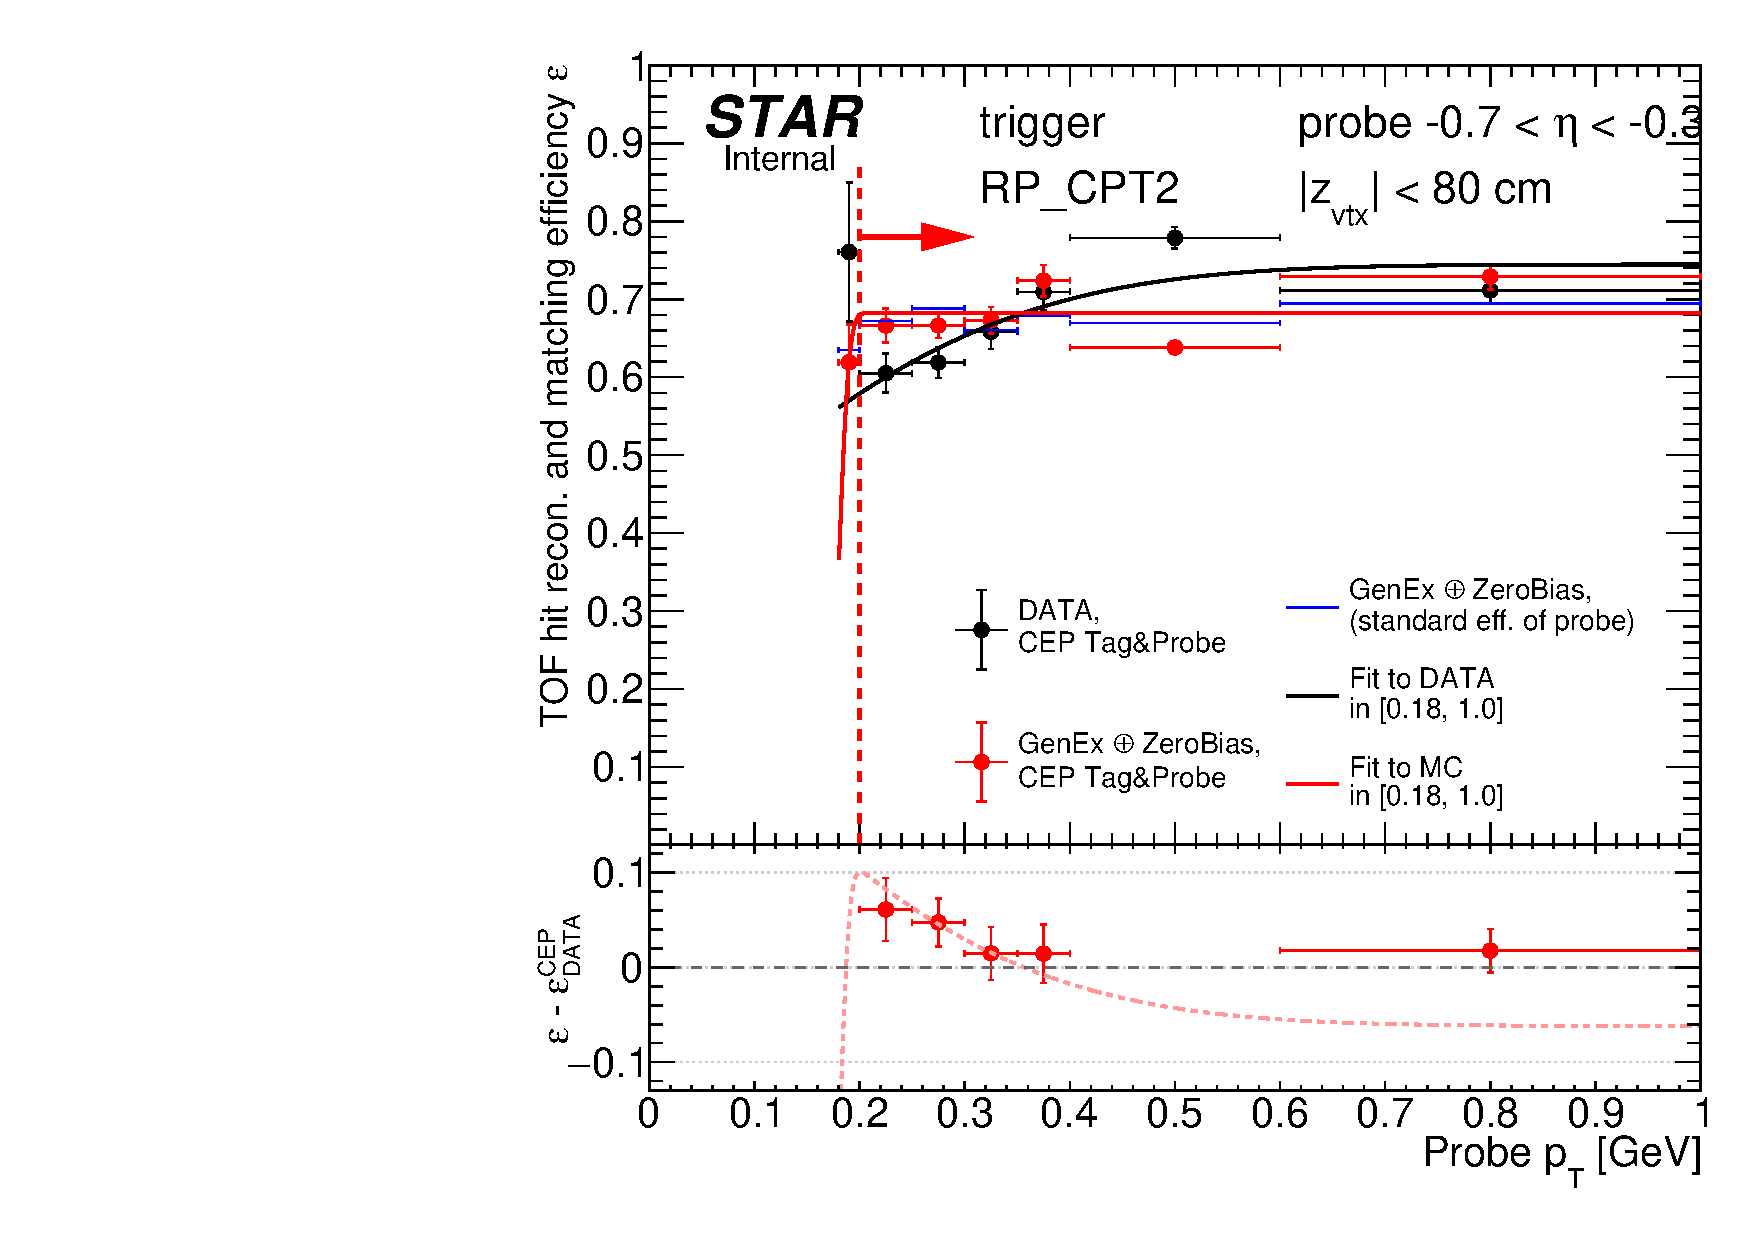
\includegraphics[width=\linewidth]{graphics/correctionsToEff/TOF_tagAndProbe/TofEffVsPt_eta_minus07_to_minus03.CPT2.pdf}\vspace{-5pt}}}
  \end{subfigure}\\[3pt]
  \begin{subfigure}[b]{\linewidth}\addtocounter{subfigure}{1}{
                \subcaptionbox{\label{fig:TofEffVsPt_eta_plus03_to_0}}{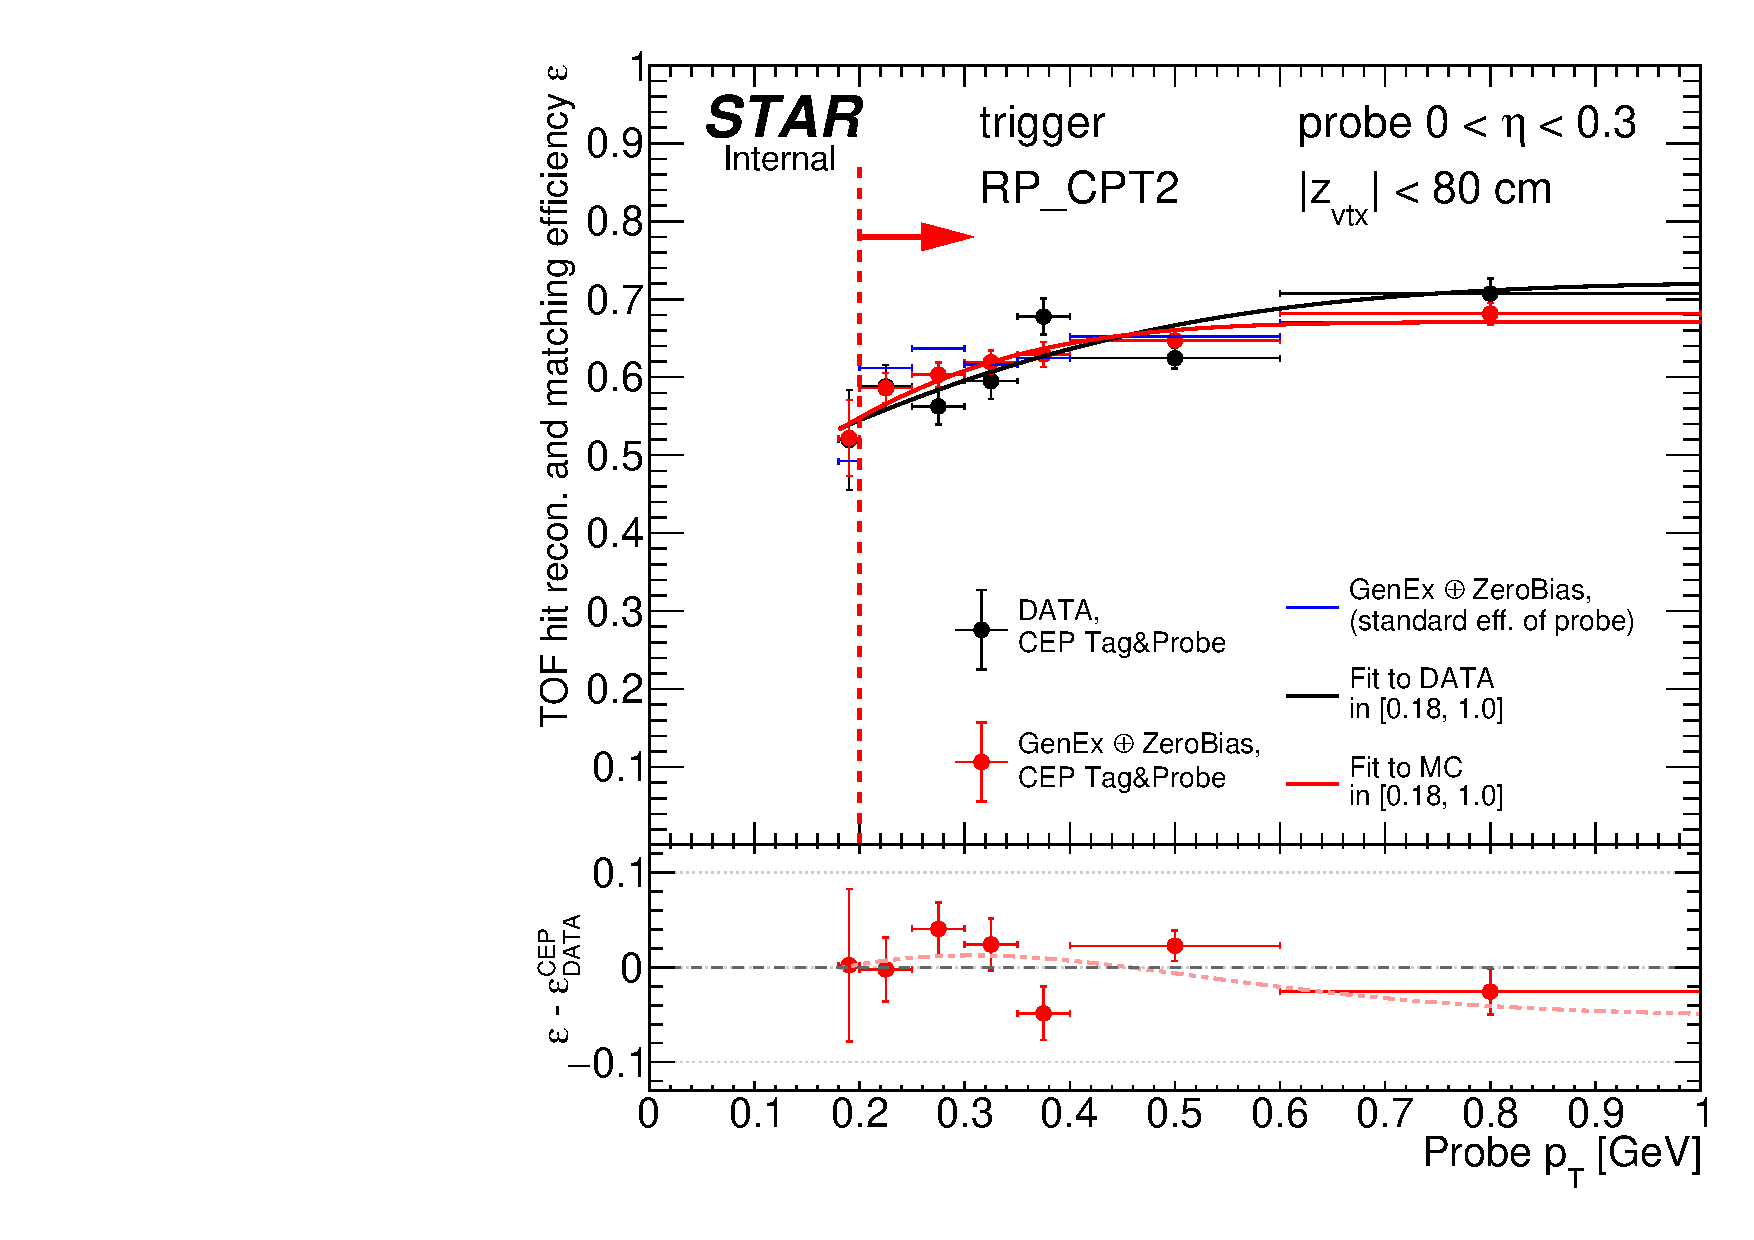
\includegraphics[width=\linewidth]{graphics/correctionsToEff/TOF_tagAndProbe/TofEffVsPt_eta_plus03_to_0.CPT2.pdf}\vspace{-5pt}}}
  \end{subfigure}
}
\quad
\parbox{0.4725\textwidth}{
  \centering
  \begin{subfigure}[b]{\linewidth}\addtocounter{subfigure}{-2}{
                \subcaptionbox{\label{fig:TofEffVsPt_eta_minus03_to_0}}{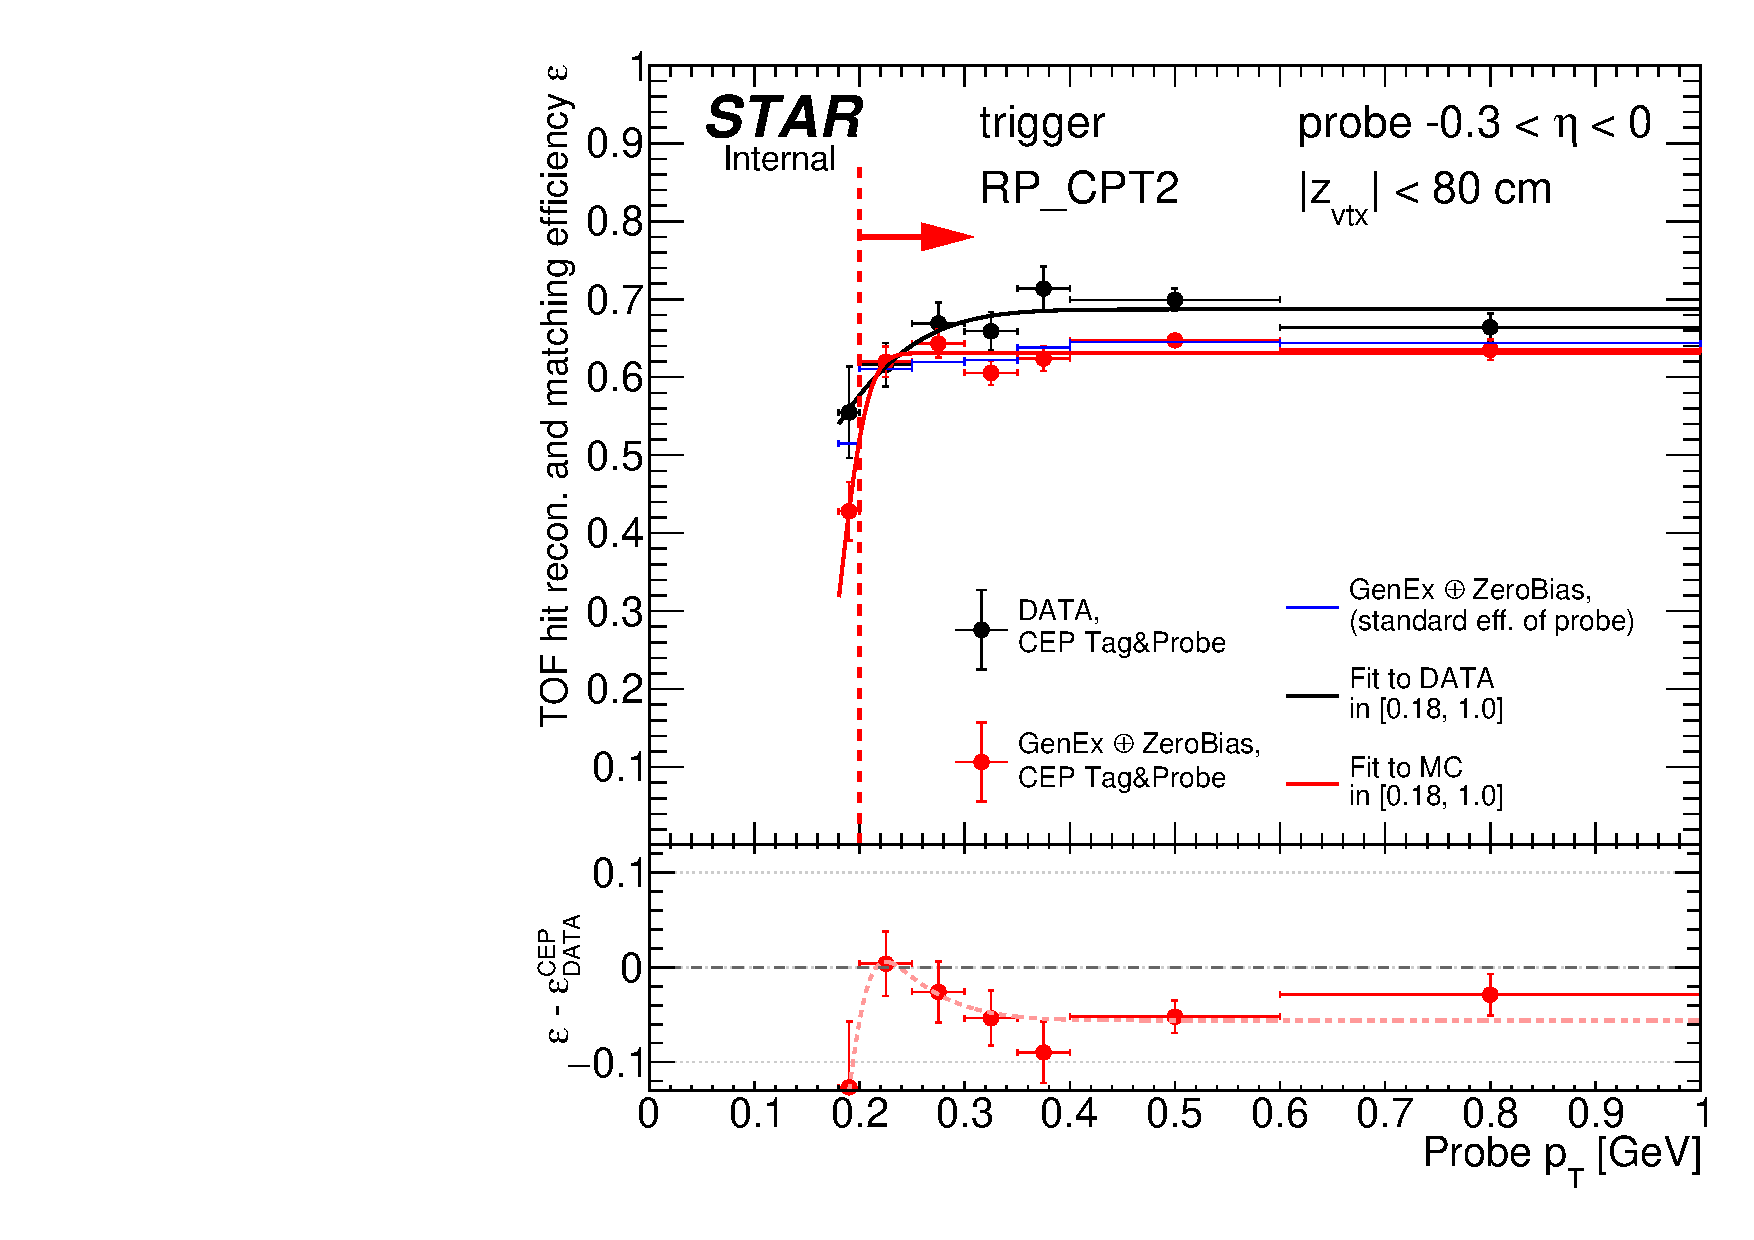
\includegraphics[width=\linewidth]{graphics/correctionsToEff/TOF_tagAndProbe/TofEffVsPt_eta_minus03_to_0.CPT2.pdf}\vspace{-5pt}}}
  \end{subfigure}\\[3pt]
  \begin{subfigure}[b]{\linewidth}\addtocounter{subfigure}{1}{
                \subcaptionbox{\label{fig:TofEffVsPt_eta_plus07_to_plus03}}{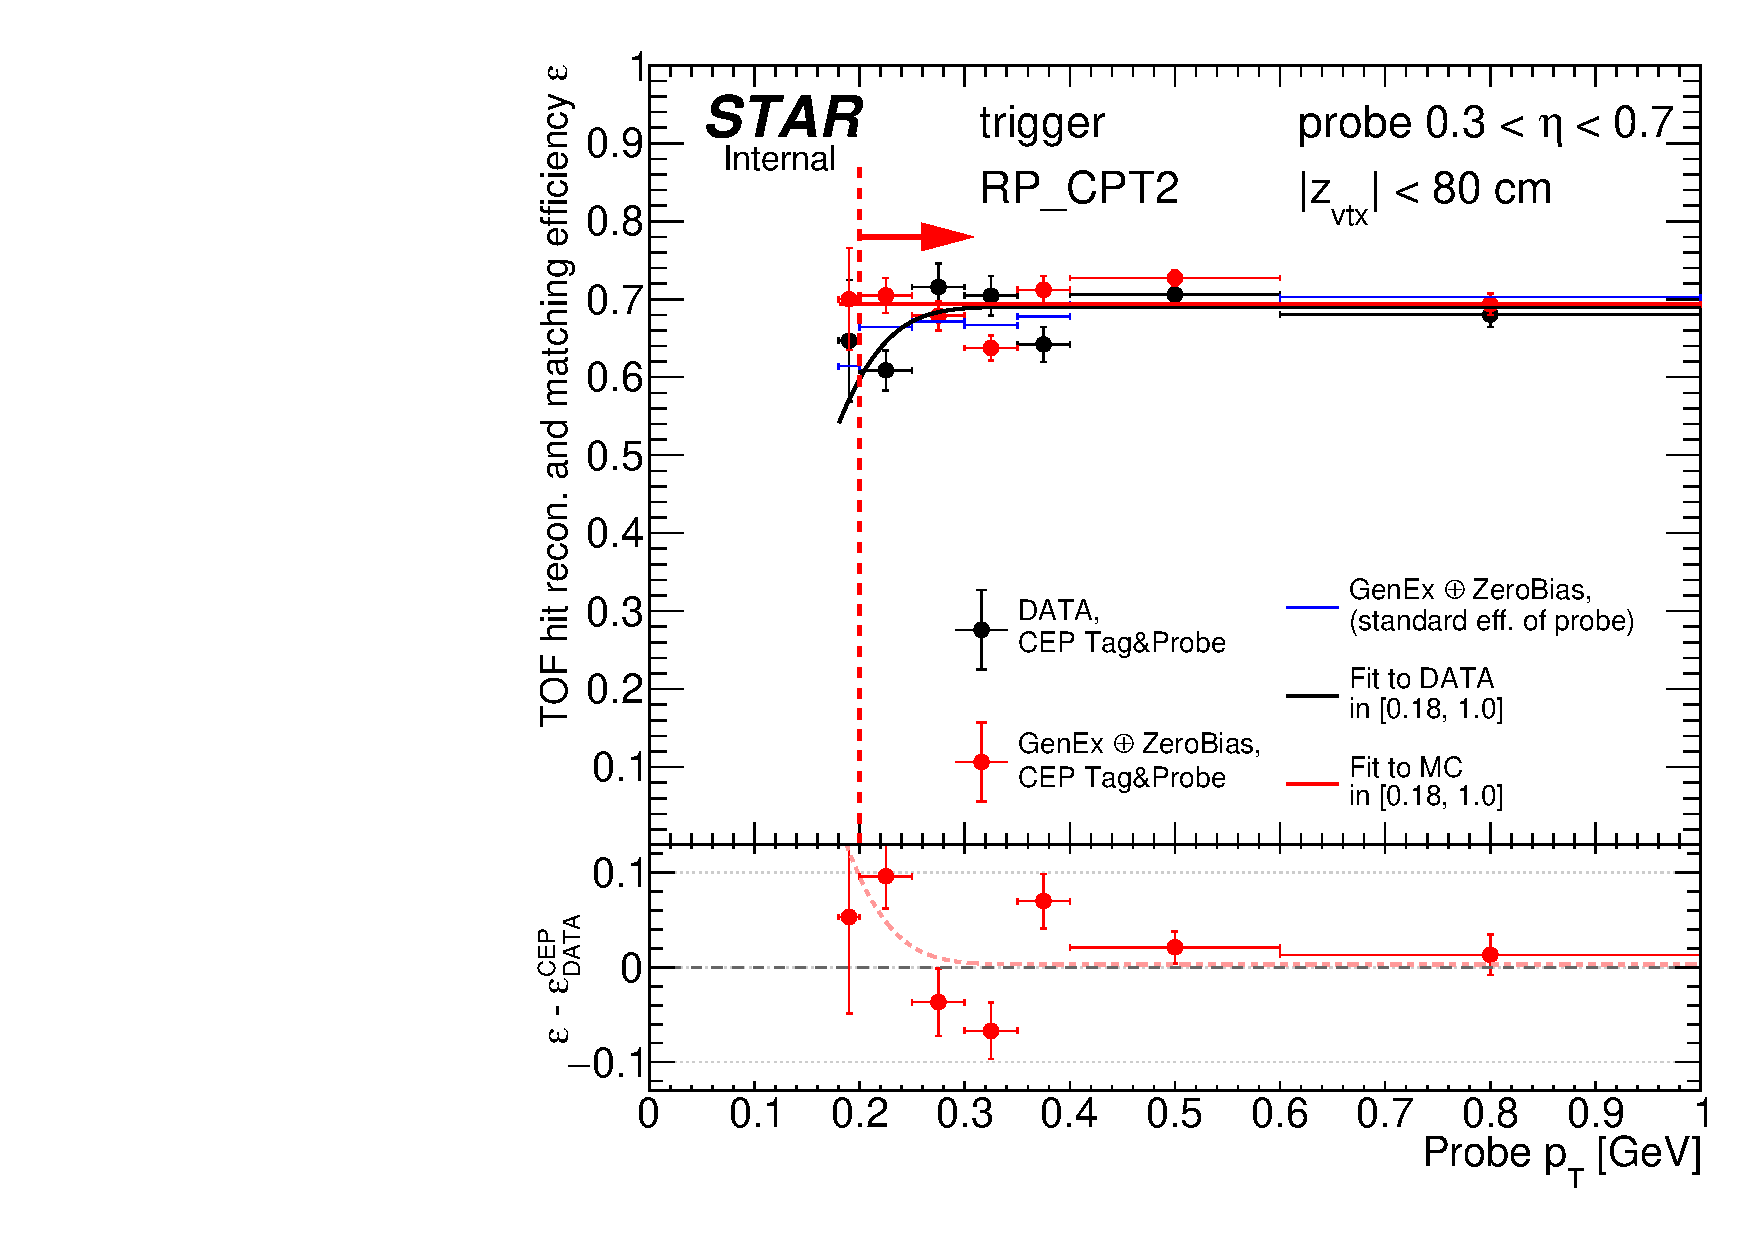
\includegraphics[width=\linewidth]{graphics/correctionsToEff/TOF_tagAndProbe/TofEffVsPt_eta_plus07_to_plus03.CPT2.pdf}\vspace{-5pt}}}
  \end{subfigure}
}%\vspace{-5pt}%
\caption[Tag\&Probe TOF efficiency from CEP data compared with the result from embedded CEP MC (divided w.r.t. $\eta$ of the probe).]%
    {Tag\&Probe TOF efficiency from CEP data (black points) compared with the result from embedded CEP MC (red points) as a function of TPC track $p_{T}$ for four ranges of the pseudorapidity $\eta$ of the probe. Blue lines denote the TOF efficiency calculated in the standard way solely from the selected probe tracks that were matched to primary pions at the true level. Difference between red points and blue lines show the potential bias of tag and probe method. Solid lines are fits of function given by Eq.~\eqref{eq:tofEffFunc} to points of corresponding color, whose parameters are tabulated in Tab.~\ref{tab:tofEffCorrParams}. Dashed vertical lines with arrows indicate region of $p_{T}$ and $\eta$ accepted in analyses.}\label{fig:tofEffSyst_etaBins}%
\end{figure}%
%---------------------------
%
%
%
%
\noindent where $\varepsilon^{\text{TOF}}_{\text{DATA}}(p_{T})$ and $\varepsilon^{\text{TOF}}_{\text{MC}}(p_{T})$ are of the form given by Eq.~\eqref{eq:tofEffFunc} with parameters from Tab.~\ref{tab:tofEffCorrParams} for the data and MC, respectively. The same correction is used for positive and negative charge particles.

Due to much lower statistics a similiar study cannot be performed for kaons and protons. We therefore apply the same correction $\delta\varepsilon^{\text{TOF}}(p_{T})$ to the TOF efficiency for $K^{\pm}$ and $p(\bar{p})$.

After our study of systematic uncertainty of the TOF efficiency we decided to introduce another correction, on top of the correction derived in this Section. This additional corection was introduced in order to symetrize systematic unceratinty on the TOF efficiency, as described in Sec.~\ref{subsec:tofAbsEffSystAndCorr}.
 

\begin{table}[t!]%
\centering%
\begin{tabular}{c||r|r|r||r|r|r}%\hline
\multirow{2}{*}{\textbf{\bm{$\eta$} range}} &  \multicolumn{3}{c||}{\textbf{Data}} & \multicolumn{3}{c}{\textbf{MC}} \\ \cline{2-7}
  & \multicolumn{1}{c|}{$P_{1}$} & \multicolumn{1}{c|}{$P_{2}$} & \multicolumn{1}{c||}{$P_{3}$} & \multicolumn{1}{c|}{$P_{1}$} & \multicolumn{1}{c|}{$P_{2}$} & \multicolumn{1}{c}{$P_{3}$} \\ \Xhline{2\arrayrulewidth}
$[-0.7; -0.3]$   &\small  $ 0.736 \pm 0.011 $  &\small  $ 0.013 \pm 0.083 $  &\small  $ 0.329 \pm 0.106 $  &\small  $ 0.686 \pm 0.010 $  &\small  $ 0.180 \pm 0.036 $  &\small  $ 0.011 \pm 0.039 $\\
$[-0.3; ~~0.0]$   &\small  $ 0.696 \pm 0.011 $  &\small  $ 0.090 \pm 0.070 $  &\small  $ 0.164 \pm 0.079 $  &\small  $ 0.629 \pm 0.003 $  &\small  $ 0.180 \pm 0.004 $  &\small  $ 0.029 \pm 0.011 $\\
$[~0.0; ~~0.3]$   &\small  $ 0.716 \pm 0.031 $  &\small  $ -0.050 \pm 0.137 $  &\small  $ 0.508 \pm 0.233 $  &\small  $ 0.670 \pm 0.005 $  &\small  $ -0.021 \pm 0.096 $  &\small  $ 0.344 \pm 0.154 $\\
$[~0.3;~~ 0.7]$   &\small  $ 0.683 \pm 0.008 $  &\small  $ 0.132 \pm 0.055 $  &\small  $ 0.084 \pm 0.056 $  &\small  $ 0.690 \pm 0.009 $  &\small  $ 0.167 \pm 0.002 $  &\small  $ 0.000 \pm 0.000 $\\
\end{tabular}%
\caption[Parameters of function describing the TOF efficiency as a function of pion track $p_{T}$ in bins of track $\eta$.]{Parameters of function (Eq.~\eqref{eq:tofEffFunc}) describing the TOF efficiency as a function of pion track $p_{T}$ in bins of track $\eta$ from Fig.~\ref{fig:tofEffSyst_etaBins}. Paramaters of the functions fitted to both data and MC points are given. The TOF efficiency calculated as described in Sec.~\ref{sec:tofMatchEff} is corrected during data analysis by the difference of values of functions $\varepsilon^{\text{TOF}}(p_{T})$ with parameters for data and MC, respectively (the difference is added).}\label{tab:tofEffCorrParams}
\end{table}





\section{Data driven corrections to TPC efficiency}\label{sec:tpcEffCorr}


%---------------------------
\begin{figure}[h]
\centering
\parbox{0.4725\textwidth}{
  \centering
  \begin{subfigure}[b]{\linewidth}{
                \subcaptionbox{\label{fig:DaysBefore75_TpcEffVsEta}}{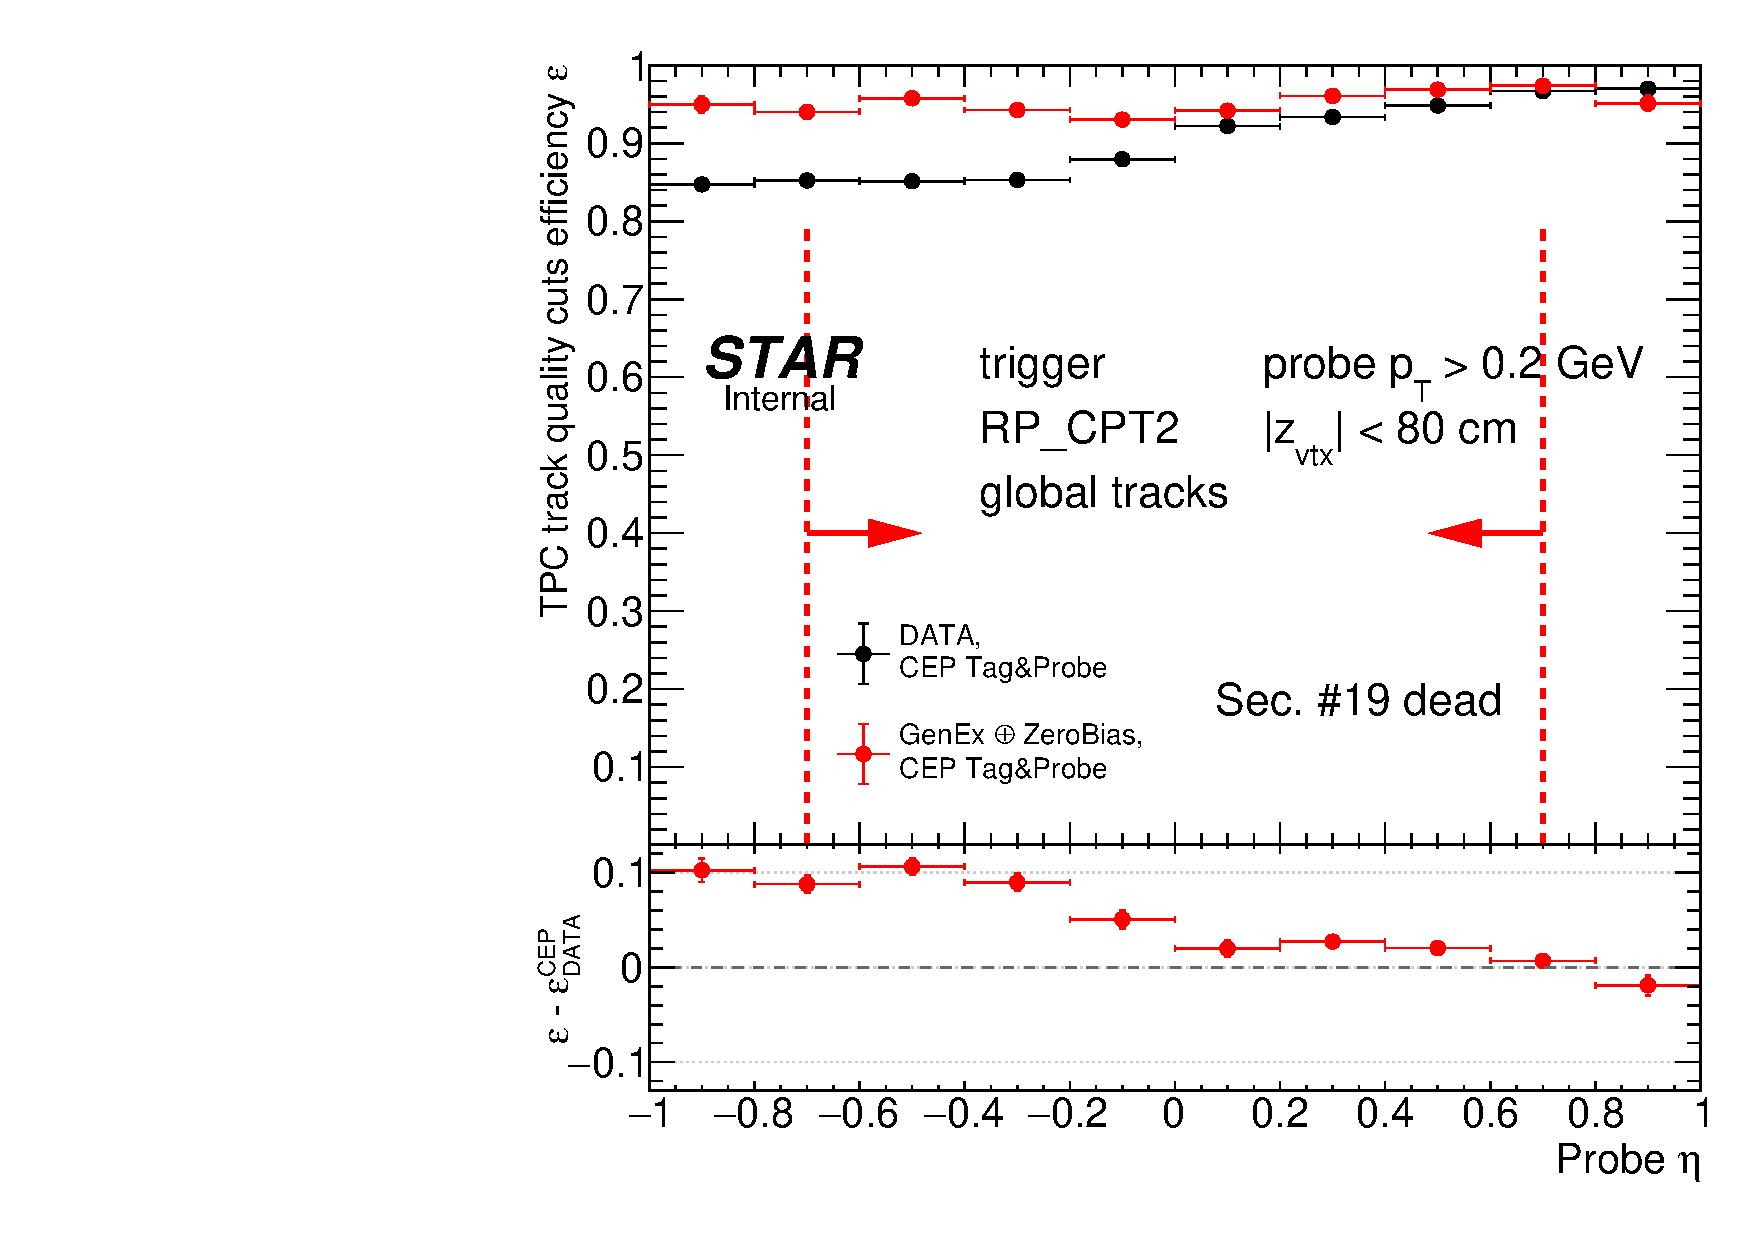
\includegraphics[width=\linewidth]{graphics/correctionsToEff/TPC_tagAndProbe/DaysBefore75_TpcEffVsEta.CPT2.pdf}\vspace{-5pt}}}
  \end{subfigure}
}
\quad
\parbox{0.4725\textwidth}{
  \centering
  \begin{subfigure}[b]{\linewidth}{
                \subcaptionbox{\label{fig:DaysAfter75_TpcEffVsEta}}{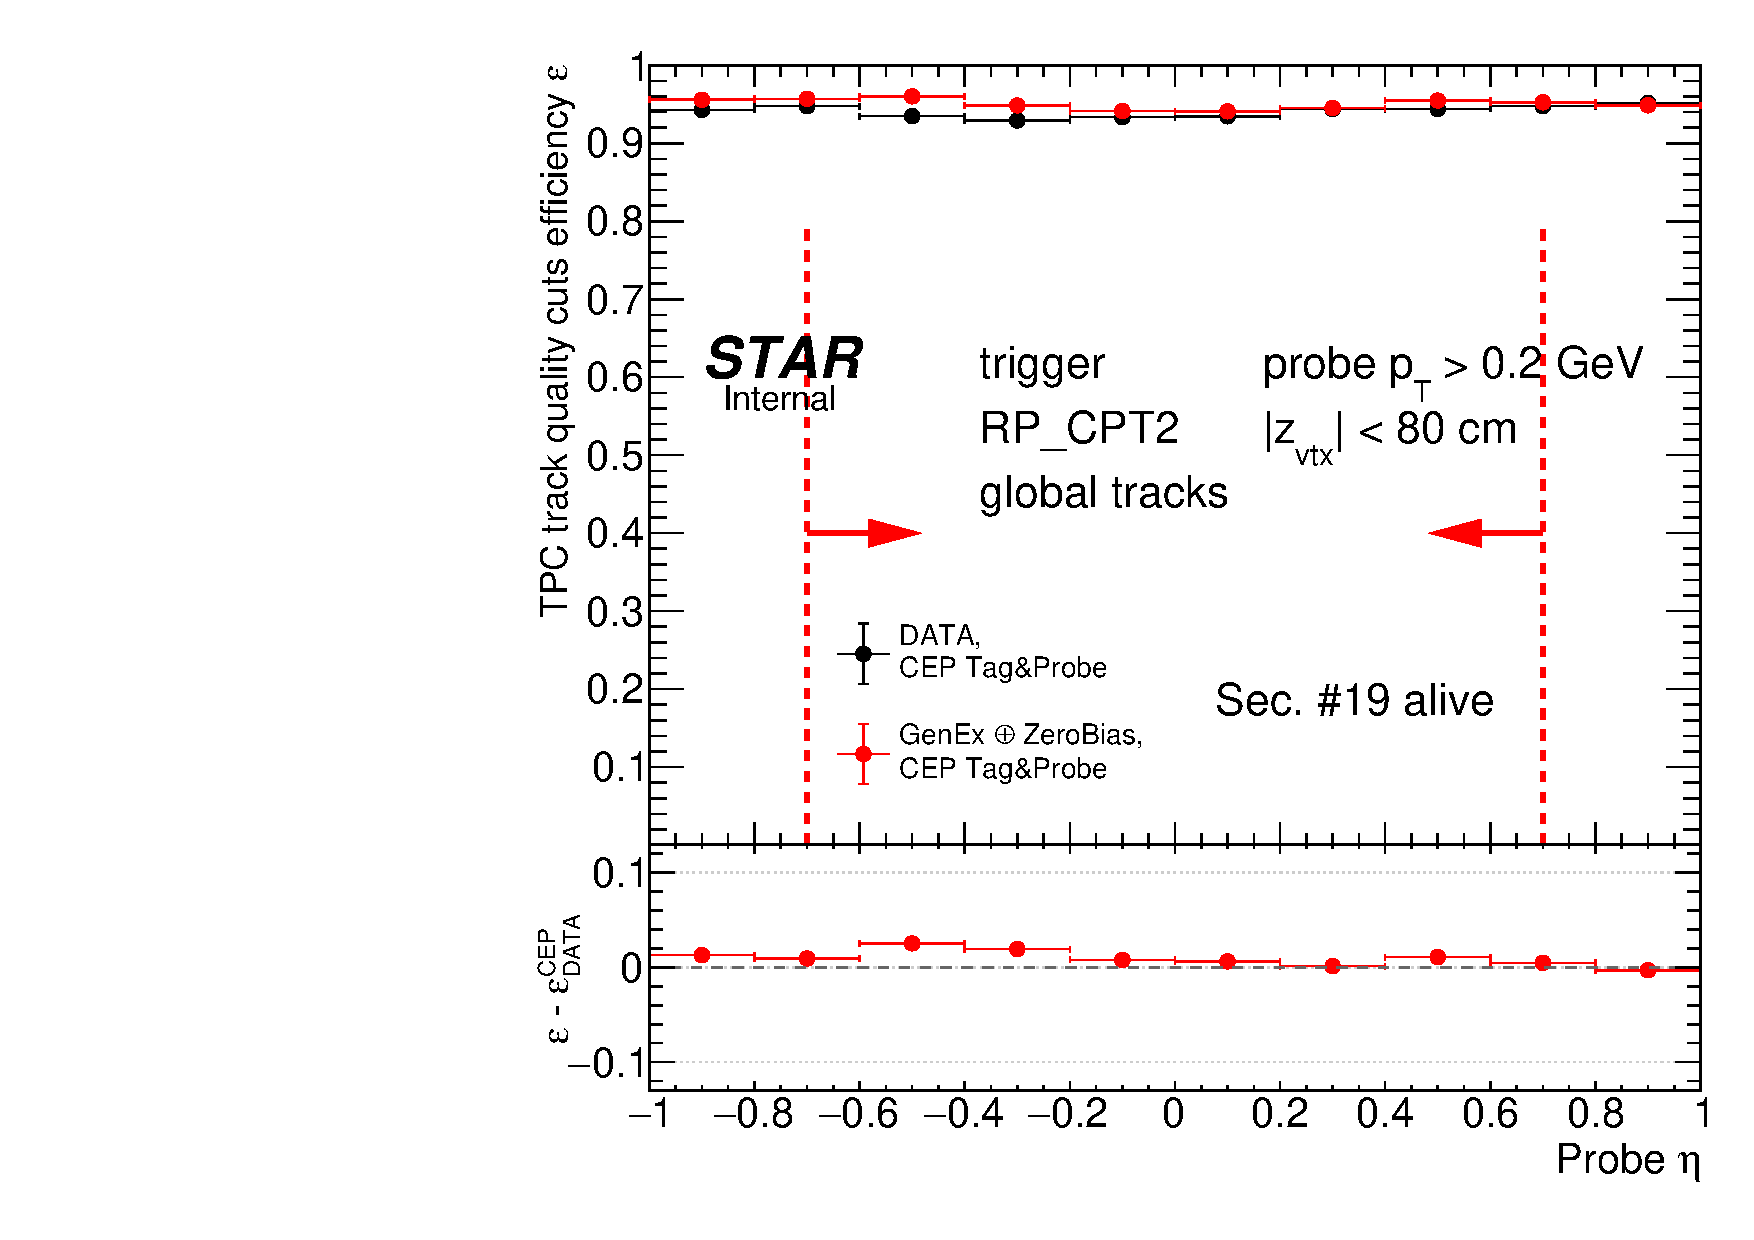
\includegraphics[width=\linewidth]{graphics/correctionsToEff/TPC_tagAndProbe/DaysAfter75_TpcEffVsEta.CPT2.pdf}\vspace{-5pt}}}
  \end{subfigure}
}%\vspace{-5pt}%
\caption[Tag\&Probe TPC track selection efficiency from CEP data compared with the result from embedded CEP MC.]%
    {Tag\&Probe TPC track selection efficiency from CEP data (black points) compared with the result from embedded CEP MC (red points) as a function of TPC track $\eta$. %Solid lines are fits of function given by Eq.~\eqref{eq:tofEffFunc} to points of corresponding color, whose parameters are tabulated in Tab.~\ref{tab:tofEffCorrParams}. Dashed vertical lines with arrows indicate region of $p_{T}$ and $\eta$ accepted in analyses.
    }\label{fig:tofEffSyst_etaBins}% 
\end{figure}%
%---------------------------





\section{Data driven corrections to RP efficiency}\label{sec:rpTrackEffCorr}

Study of systematic uncertainty of the RP track reconstruction efficiency revealed that in some part of the fiducial area of RP detectors a correction needs to be applied to the efficiency obtained from the MC simulation.  The details can be found in in Sec.~\ref{subsec:rpTrackRecoEffSyst}. 
